\documentclass[aspectratio=169]{beamer}

\usepackage[utf8]{inputenc}

\usepackage{amsfonts}
\usepackage{amsmath}
\usepackage{color}
\usepackage{listings}
\usepackage{tikz}
\usepackage{hyperref}

\newif\ifnotes
%  \notestrue
  \notesfalse

\newif\iftransitions
% \transitionstrue
 \transitionsfalse

\newif\iffast
% \fasttrue
  \fastfalse

\ifnotes
\usepackage{pgfpages}
\setbeameroption{show notes}
\setbeameroption{show notes on second screen=right}
\fi

\usetheme{Rochester}
\usecolortheme{beaver}

\addtobeamertemplate{navigation symbols}{}{%
    \usebeamerfont{footline}%
    \usebeamercolor[fg]{footline}%
    \hspace{1em}%
    \insertframenumber/\inserttotalframenumber
}

\lstloadlanguages{C++}
    \lstset{%
        language={C++},
        basicstyle=\ttfamily,
        keywordstyle=\color{blue},
        showstringspaces=false,
        escapechar={§},
        escapeinside={(*@}{@*)}
    }

\lstdefinestyle{cpp20}{language={C++},
  morekeywords={noexcept,co_await,co_return,co_yield,requires,consteval,constinit,concept,module,export,import}
}

\lstdefinestyle{cmake}{
  morekeywords={add_executable,add_library,cmake_minimum_required,project,target_include_directories,target_link_libraries,target_sources}
}

\tikzstyle{every picture}+=[remember picture]

\newcommand{\cpause}{\iftransitions \pause \fi}

\newcommand{\cuncover}[2]{\iftransitions \uncover<#1>{#2} \else #2 \fi}

\newcommand{\tmrk}[2]{\tikz[baseline,inner sep=0]\node[anchor=base](#1){#2};}

\title{C++ Modules - Getting Started Today}
\author{Andreas Weis}
\institute{Woven by Toyota}

\date{CppCon 2023}
\titlegraphic{
\includegraphics[height=.15\textheight]{resources/cppcon.png}}

\iffalse
Modules have been one of the most highly anticipated features of C++20. Unfortunately, it was also the language feature that took the longest to become widely available for developers to use. This year for the first time we see broad support for the feature in all major compilers and mainstream build system support through CMake. The goal of this talk is to provide you with all the basic knowledge to allow you getting started with C++20 modules today.

We will take a look at how modules change the build process and why it took so long to implement them. We will take a tour of the essentials of the named modules mechanism and explore the new best practices for physical code structure in a modules-based code base, including how to set up a build with CMake. And last but not least, we will discuss different options for interacting with existing header-based code.

The talk will focus above all else on practicality: We will only be covering features that are widely available for use today with the latest compilers and build tools. We will give special attention to the areas where the design practices for modules differ from the familiar header-based approach and address common misconceptions and pitfalls that are typical among developers first encountering the feature. No prior knowledge of modules is required.

Outline:
* Modules "Hello World" example
* Differences module interfaces vs header files
* Understanding the build process for modules
* Build system support with CMake and Ninja/MSBuild
* Modules with static and shared libraries
* Best practices for code structure with modules
* Migrating legacy code
* The modularized standard library
* Wrapping third-party code in named modules interfaces

Comments:
This talk aims for breadth not depth. The intention is to give an overview of all the essential topics that are useful when picking up modules for the first time, while not going into as much detail as the more specialized talks we saw at CppCon in the past.

Sections:
5-12 Include World      7 (0:01)
13-28 Hello Modules    15 (0:05)
29-37 Types of Modules  8 (0:15)
38-47 CMake             9 (0:25)
48-65 Build systems    17 (0:35)
66-83 Best practices   17 (0:45)
Wrapup                  2 (0:55)
\fi

\begin{document}

% cover slide
{ % all template changes are local to this group.
    \setbeamertemplate{navigation symbols}{}
    \begin{frame}<article:0>[plain]
        \begin{tikzpicture}[remember picture,overlay]
            \node[at=(current page.center)] {
                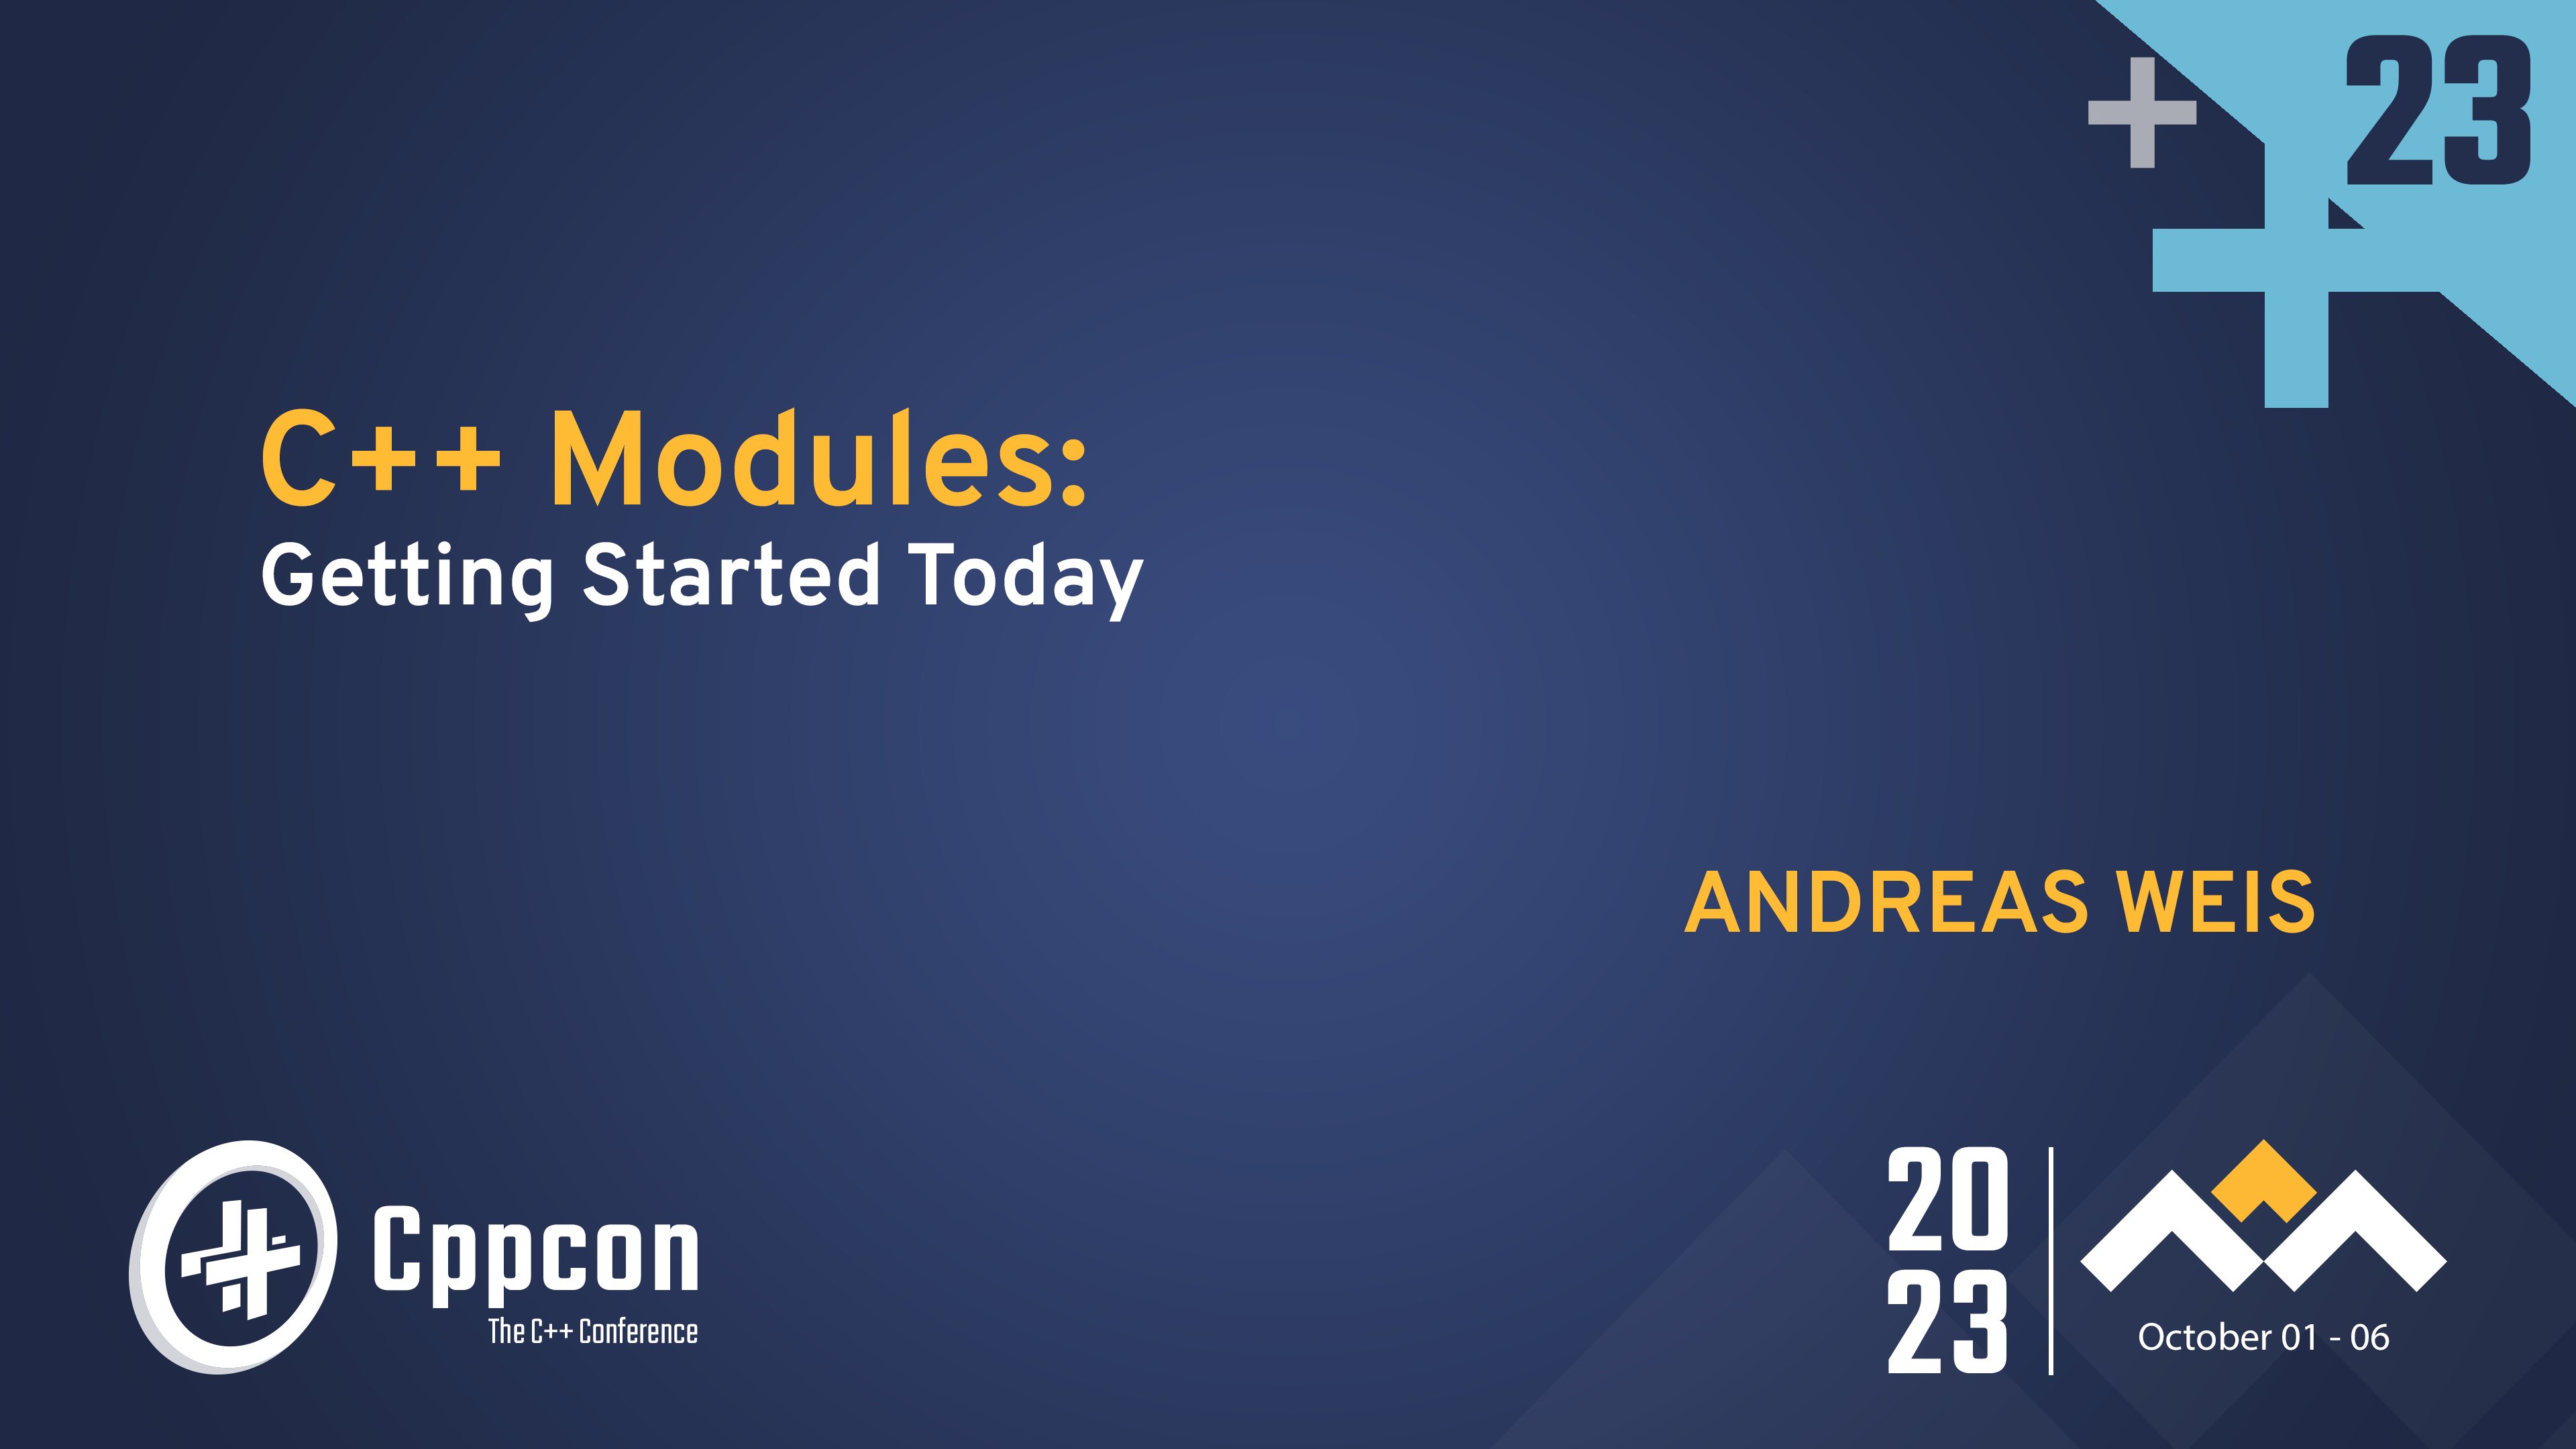
\includegraphics[keepaspectratio,
                                 width=\paperwidth,
                                 height=\paperheight]{modulesgfx/titlecard_cppcon.png}
            };
        \end{tikzpicture}
     \end{frame}
}
\addtocounter{framenumber}{-1}

\frame{\titlepage}

\iftrue %crop
\fi

\begin{frame}
  \frametitle{Introduction}

  \note{
  This is an introductory talk for people who have never used modules.
  The goal of this talk is to help you getting started to try out modules on your own for the first time.
  You will not learn everything you need to know about modules here. I will omit several things and simplify explanations to focus on what is most useful when starting out. My hope is that this will be a good starting point from which you can proceed deeper into the topic.

  We are going to focus on the mechanisms that are available in implementations today, that is, named modules. We are not going to cover some of the more advanced features, or features for which implementation support is still particularly bad today.

  I submitted this talk because I wanted to provide a \textit{first talk to watch} about modules that covers all the basics without assuming prior knowledge. There are many excellent second talks to watch and you should watch them. I will refer to some in this presentation which I found useful, and you will find others during this week at the conference.
  }
\end{frame}

\begin{frame}[fragile]
  \frametitle{About me - Andreas Weis (he/him)}

  \begin{itemize}
    \setlength\itemsep{1.5em}

    \item \href{https://stackoverflow.com/users/577603/comicsansms}{
\includegraphics[height=.05\textheight]{resources/so-icon.png}} \href{https://github.com/ComicSansMS}{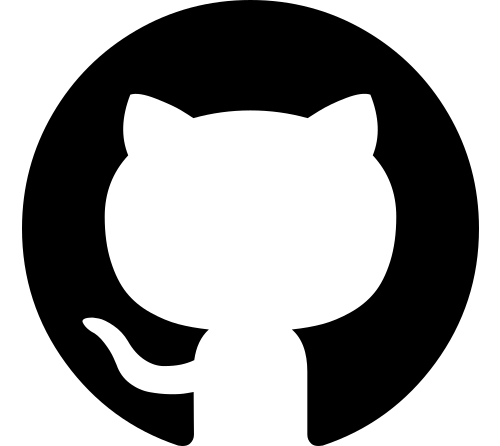
\includegraphics[height=.05\textheight]{resources/github-icon.png}} \includegraphics[height=.05\textheight]{resources/discord-icon.png} ComicSansMS

    %\item \href{https://twitter.com/DerGhulbus/}{
\includegraphics[height=.05\textheight]{resources/twitter-icon.png} @DerGhulbus}

    \item 
\includegraphics[height=.05\textheight]{resources/meetup-icon.png} Co-organizer of the \href{https://www.meetup.com/MUCplusplus/}{Munich C++ User Group}

    \item Currently working as a Vehicle Architect for Woven by Toyota \includegraphics[height=.1\textheight]{resources/woven_toyota_logo.png}

  \end{itemize}
\end{frame}

\iffalse
\begin{frame}
  \frametitle{Overview}
  \begin{itemize}
    \item Categorization of precondition violations
    \item Leveraging the type system to prevent precondition violations
    \item Techniques for restricting access to data
    \item Techniques for restricting control flow
    \end{itemize}
\end{frame}
\fi

\begin{frame}[fragile]
  \frametitle{A familiar example...}

  --- \textit{File:} \texttt{my\_function.hpp}
  \begin{lstlisting}[style=cpp20]
char const* my_function();
  \end{lstlisting}

  --- \textit{File:} \texttt{my\_function.cpp}
  \begin{lstlisting}[style=cpp20]
char const* my_function() {
  return "Hello from function!";
}
  \end{lstlisting}

  \cpause
  --- \textit{File:} \texttt{main.cpp}
  \begin{lstlisting}[style=cpp20]
#include <my_function.hpp>
#include <print>

int main() {
  std::println("{}", my_function());
}
  \end{lstlisting}

  \note{
  Just a normal header/cpp sample.
  \begin{itemize}
    \item Interface/Implementation
    \item Client
  \end{itemize}

  }
\end{frame}

\begin{frame}[fragile]
  \frametitle{\texttt{\#include} can happen anywhere}
  --- \textit{File:} \texttt{a.hpp}
  \begin{lstlisting}[style=cpp20]
inline int my_function
#include <a_impl.hpp>
  \end{lstlisting}

  --- \textit{File:} \texttt{a\_impl.hpp}
  \begin{lstlisting}[style=cpp20]
{
  return 42;
}
  \end{lstlisting}

  \note{
  Problem: include in weird places
  }
\end{frame}


\begin{frame}[fragile]
  \frametitle{Including files twice does not work}

  --- \textit{File:} \texttt{a.hpp}
  \begin{lstlisting}[style=cpp20]
class A {};
  \end{lstlisting}

  --- \textit{File:} \texttt{main.cpp}
  \begin{lstlisting}[style=cpp20]
#include <a.hpp>
#include <a.hpp>  // redefiniton error!

int main() {
}
  \end{lstlisting}

  \note{
  Problem: include guards
  }
\end{frame}

\begin{frame}[fragile]
  \frametitle{Included files are not isolated from the surrounding state}

  --- \textit{File:} \texttt{a.hpp}
  \begin{lstlisting}[style=cpp20]
class A {
private:
  char const* u_cant_touch_this() {
    return "Preprocessor hits me so hard";
  }
};
  \end{lstlisting}
  \cpause
  --- \textit{File:} \texttt{main.cpp}
  \begin{lstlisting}[style=cpp20]
#define private public
#include <a.hpp>
#undef private
int main() {
  std::println("{}", A{}.u_cant_touch_this());
}
  \end{lstlisting}

  \note{
  Problem: x-macros
  }
\end{frame}

\begin{frame}[fragile]
  \frametitle{Included files do not need to be self-contained}

  --- \textit{File:} \texttt{a.hpp}
  \begin{lstlisting}[style=cpp20]
class A {
  std::vector<int> numbers;
};
  \end{lstlisting}

  --- \textit{File:} \texttt{main.cpp}
  \begin{lstlisting}[style=cpp20]
#include <vector>
#include <a.hpp>

int main() {
}
  \end{lstlisting}

  \note{
  Problem: include what you use
  }
\end{frame}

\begin{frame}[fragile]
  \frametitle{Include files are compiled again for each translation unit}

    --- \textit{File:} \texttt{a.cpp}
  \begin{lstlisting}[style=cpp20]
#include <massive_header.hpp>

// [...]
  \end{lstlisting}

  --- \textit{File:} \texttt{b.cpp}
  \begin{lstlisting}[style=cpp20]
#include <massive_header.hpp>

// [...]
  \end{lstlisting}

  \note{
  Problem: build performance
  }
\end{frame}

\iffalse
\begin{frame}
  \frametitle{Before we dive into modules...}

  \begin{center}
  \huge{Disclaimer}
  \end{center}
\end{frame}
\fi

\begin{frame}[fragile]
  \frametitle{Hello Modules!}

  \cpause
  --- \textit{File:} \texttt{module.cpp}
  \begin{lstlisting}[style=cpp20]
(*@\tmrk{exp01}{}@*)export module my_module;(*@\tmrk{exp02}{}@*)

export char const* my_function() {
  return "Hello Modules!";
}
  \end{lstlisting}

  \cuncover{3-}{\tikz[overlay]\filldraw[blue, opacity=0.3] ([shift={(0,-0.5ex)}]exp01) rectangle ([shift={(0,2ex)}]exp02);}

  \cpause
  \cpause

  --- \textit{File:} \texttt{main.cpp}
  \begin{lstlisting}[style=cpp20]
#include <print>
(*@\tmrk{imp01}{}@*)import my_module;(*@\tmrk{imp02}{}@*)

int main() {
  std::println("{}", my_function());
}
  \end{lstlisting}

  \cuncover{5-}{\tikz[overlay]\filldraw[blue, opacity=0.3] ([shift={(0,-0.5ex)}]imp01) rectangle ([shift={(0,2ex)}]imp02);}

  \note{
    \textbf{TIMECHECK}: 0:05
    \begin{itemize}
      \item Let's see how modules solve all these problems.
      \item This is a simple module providing just one function.
      \item Module starts with export declaration. Module name is given here. Name can be different from filename.
      \item The client side
      \item import pulls in the module. Module name needs to be unique. Module does not introduce a namespace!
    \end{itemize}
  }
\end{frame}

\begin{frame}[fragile]
  \frametitle{Exporting things}

  \begin{lstlisting}[style=cpp20]
// functions
export int getNumber();
  \end{lstlisting}
  \cpause
  \begin{lstlisting}[style=cpp20]
// types
export class SomeType;
  \end{lstlisting}
  \cpause
  \begin{lstlisting}[style=cpp20]
// templates
export template<typename T>
T combine(T n1, T n2);
export template<typename T>
class MyTemplatedType;
  \end{lstlisting}

  \note{
  We can export
  \begin{itemize}
  \item functions
  \item types
  \item templates. Export comes first!
  \end{itemize}
  We are exporting names! Names are introduced by declarations.
  }
\end{frame}

\begin{frame}[fragile]
  \frametitle{Exporting things}

  \begin{lstlisting}[style=cpp20]
export namespace a {
  void is_exported();
}
namespace a {
  void is_not_exported();
}
  \end{lstlisting}
  \cpause
  \begin{lstlisting}[style=cpp20]
namespace a {
  void will_be_exported_in_b();
}
export namespace b {
  export using ::a::will_be_exported_in_b;
}
  \end{lstlisting}

  \note{
  We can export
  \begin{itemize}
  \item Namespaces. Namespace can be (re-)opened anywhere, so export only affects current place.
  \item Using declarations. Useful for re-exporting things from components out of our control.
  \end{itemize}
  }
\end{frame}

\begin{frame}[fragile]
  \frametitle{Exporting things}

  \begin{lstlisting}[style=cpp20]
export {
  void will_be_exported();

  void will_also_be_exported();

  struct WillAlsoBeExported {
    // [...]
  };

  // the following will not compile:
  static void no_internal_linkage();
}
  \end{lstlisting}

  \note{
  We can export
  \begin{itemize}
  \item Export blocks. Don't put stuff in here that does not make sense to be exported.
  \end{itemize}
  }
\end{frame}

\begin{frame}[fragile]
  \frametitle{Exporting things}

  --- \textit{File:} \texttt{module1.cpp}
  \begin{lstlisting}[style=cpp20]
export module A;

export int foo() { return 42; }
  \end{lstlisting}
  --- \textit{File:} \texttt{module2.cpp}
  \begin{lstlisting}[style=cpp20]
export module B;

export import A;
  \end{lstlisting}
  \cpause
  --- \textit{File:} \texttt{main.cpp}
  \begin{lstlisting}[style=cpp20]
import B;
int main() {
  return foo();
}
  \end{lstlisting}

  \note{
  We can export
  \begin{itemize}
  \item Other modules. export import looks weird but makes sense.
  \item Client can access things as if part of the exporting module.
  \end{itemize}
  }
\end{frame}

\begin{frame}[fragile]
  \frametitle{Not exported does not mean unreachable}

  --- \textit{File:} \texttt{module.cpp}
  \begin{lstlisting}[style=cpp20]
export module m;
class NotExported { int i = 42; };
export NotExported getNotExported()
{ return {}; }
  \end{lstlisting}
  \cpause
  --- \textit{File:} \texttt{main.cpp}
  \begin{lstlisting}[style=cpp20]
import m;
int main() {
  int const ii = getNotExported().i;
}
  \end{lstlisting}
  \cpause
  This is not new!
  \begin{lstlisting}[style=cpp20]
auto getS()
{ struct S { int i = 42; }; return S{}; }
  \end{lstlisting}

  \note{
  \begin{itemize}
  \item Not exported but reachable.
  \item Client can use struct but does not know its name.
  \item Same as auto return.
  \end{itemize}
  }
\end{frame}

\begin{frame}
  \frametitle{Daniela Engert - The three secret spices of C++ Modules - \\ Visibility, Reachability, Linkage}
  \begin{center}
    \href{https://www.youtube.com/watch?v=l_83lyxWGtE}
    {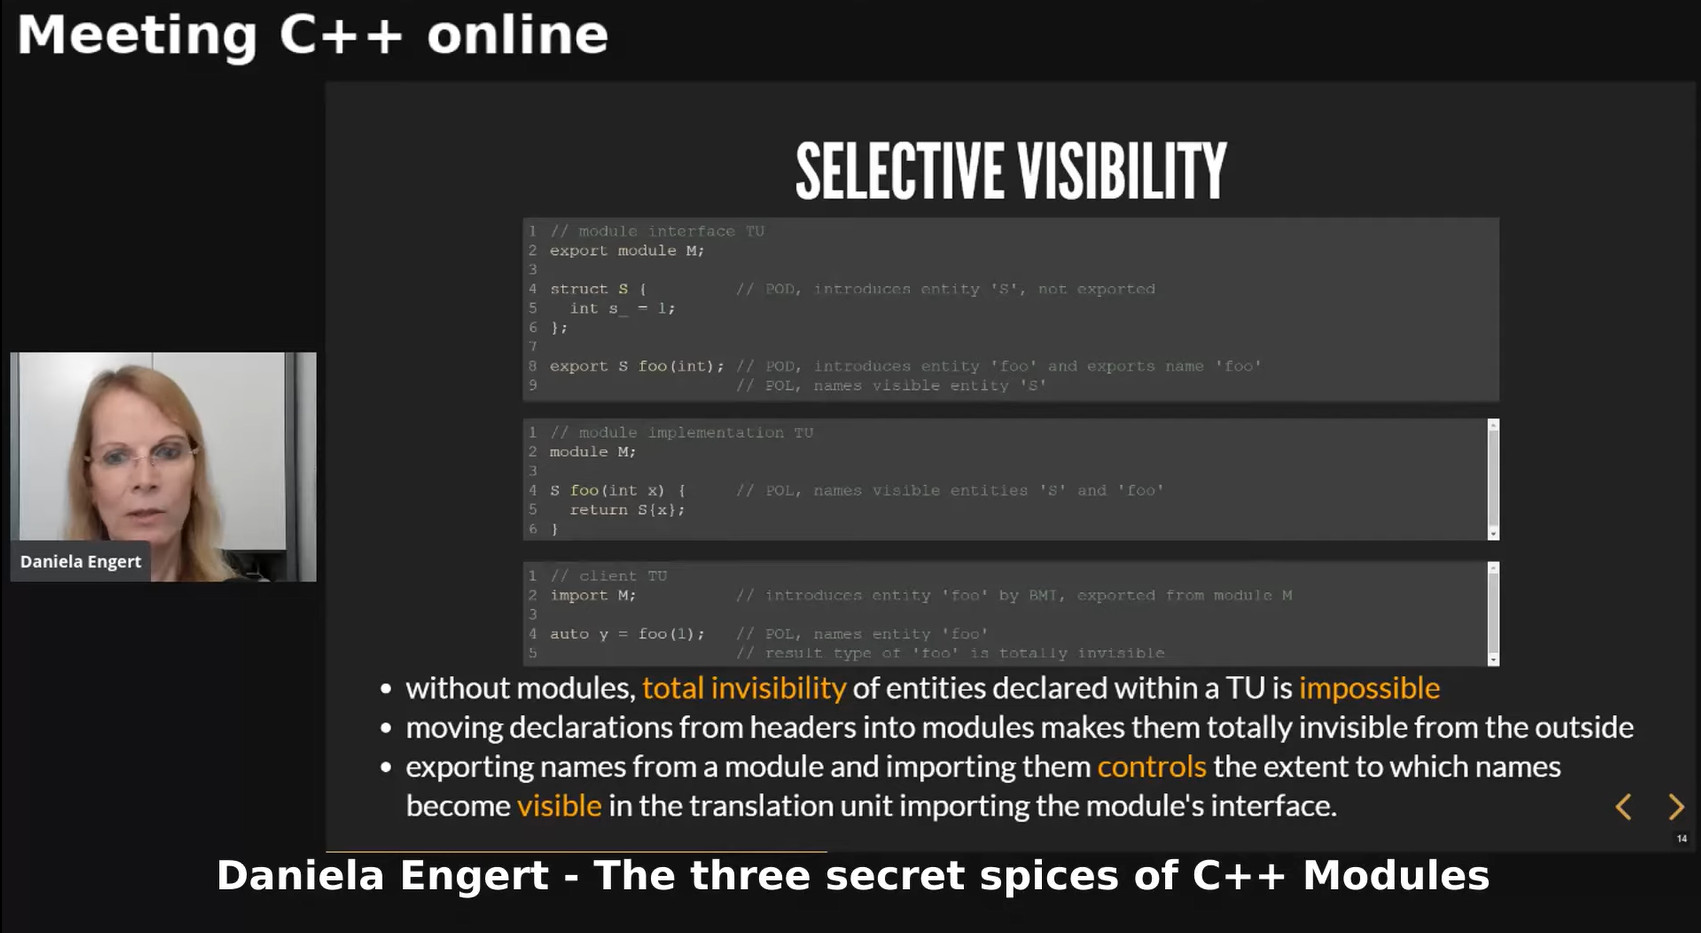
\includegraphics[height=.8\textheight]{modulesgfx/engert_three_spices.jpg}}
  \end{center}
\end{frame}

\begin{frame}
  \frametitle{Different shapes of modules}
  \note{
  \textbf{TIMECHECK}: 0:15
  }
\end{frame}

\begin{frame}[fragile]
  \frametitle{Primary Module Interface Unit}

  --- \textit{File:} \texttt{my\_module.cpp}
  \begin{lstlisting}[style=cpp20]
export module my_module;

export char const* my_function() {
  return "Hello Modules!";
}
  \end{lstlisting}

  \note{
  \begin{itemize}
  \item Primary module interface
  \begin{itemize}
    \item Primary because there can be only one for each module name
    \item By default, put everything in primary module
  \end{itemize}
  \end{itemize}
  }
\end{frame}

\begin{frame}[fragile]
  \frametitle{Module Implementation Unit}

  --- \textit{File:} \texttt{my\_module.cpp}
  \begin{lstlisting}[style=cpp20]
export module my_module;

export char const* my_function();
  \end{lstlisting}
  --- \textit{File:} \texttt{my\_module\_impl.cpp}
  \begin{lstlisting}[style=cpp20]
(*@\tmrk{a020}{}@*)module my_module;(*@\tmrk{b020}{}@*)

char const* my_function() {
  return "Hello Modules!";
}
  \end{lstlisting}

  \cpause
  \tikz[overlay]\filldraw[blue, opacity=0.3] ([shift={(0,-0.5ex)}]a020) rectangle ([shift={(0,2ex)}]b020);

  \note{
  \begin{itemize}
  \item Module implementation;
  \item Module declaration without export; Export only on declaration in interface, not in implementation; compile error otherwise
    \begin{itemize}
    \item Like Headers, as many implementations as we want
    \item Unlike Headers, no need to split
    \item Impl can change without rebuilding clients of interface
    \end{itemize}
  \end{itemize}
  }
\end{frame}

\begin{frame}[fragile]
  \frametitle{Module Interface Partitions}

  --- \textit{File:} \texttt{my\_module.cpp}
  \begin{lstlisting}[style=cpp20]
export module mice;

(*@\tmrk{a030}{}@*)export import :pinky;(*@\tmrk{b030}{}@*)
(*@\tmrk{a031}{}@*)export import :the_brain;(*@\tmrk{b031}{}@*)
  \end{lstlisting}

  \cpause
  --- \textit{File:} \texttt{my\_module\_p1.cpp}
  \begin{lstlisting}[style=cpp20]
export module (*@\tmrk{a032}{}@*)m:pinky(*@\tmrk{b032}{}@*);
export void narf() {}
  \end{lstlisting}

  --- \textit{File:} \texttt{my\_module\_p2.cpp}
  \begin{lstlisting}[style=cpp20]
export module (*@\tmrk{a033}{}@*)m:the_brain(*@\tmrk{b033}{}@*);
export void take_over_the_world() {}
(*@\tmrk{a034}{}@*)struct SecretMasterplan {}(*@\tmrk{b034}{}@*);
  \end{lstlisting}

  \iftransitions
  \only<1-2>{\tikz[overlay]\filldraw[blue, opacity=0] ([shift={(0,-0.5ex)}]a030) rectangle ([shift={(0,2ex)}]b030);}
  \only<3>{\tikz[overlay]\filldraw[blue, opacity=0.3] ([shift={(0,-0.5ex)}]a030) rectangle ([shift={(0,2ex)}]b030);}
  \only<3>{\tikz[overlay]\filldraw[blue, opacity=0.3] ([shift={(0,-0.5ex)}]a031) rectangle ([shift={(0,2ex)}]b031);}
  \only<2>{\tikz[overlay]\filldraw[blue, opacity=0.3] ([shift={(0,-0.5ex)}]a032) rectangle ([shift={(0,2ex)}]b032);}
  \only<2>{\tikz[overlay]\filldraw[blue, opacity=0.3] ([shift={(0,-0.5ex)}]a033) rectangle ([shift={(0,2ex)}]b033);}
  \only<4>{\tikz[overlay]\filldraw[blue, opacity=0.3] ([shift={(0,-0.5ex)}]a034) rectangle ([shift={(0,2ex)}]b034);}
  \fi

  \note{
  \begin{itemize}
  \item Split Module interface into multiple files;
  \item Each mouse gets its own file
  \begin{itemize}
    \item Partition is internal to module only;
  \end{itemize}
  \item All partition interfaces need to be exported by primary interface (NDR!)
  \begin{itemize}
    \item Partitions can be interface or implementation
    \item Implementation would be without export
  \end{itemize}
  \item Everyone in \texttt{mice} can see the SecretMasterplan
  \begin{itemize}
    \item But clients can not
    \item What happens if Pinky also has a SecretMasterplan?
  \end{itemize}
  \end{itemize}
  }
\end{frame}

\begin{frame}
  \frametitle{We're not talking about Header Units}

  \begin{center}
    \href{https://www.youtube.com/watch?v=_LGR0U5Opdg}
    {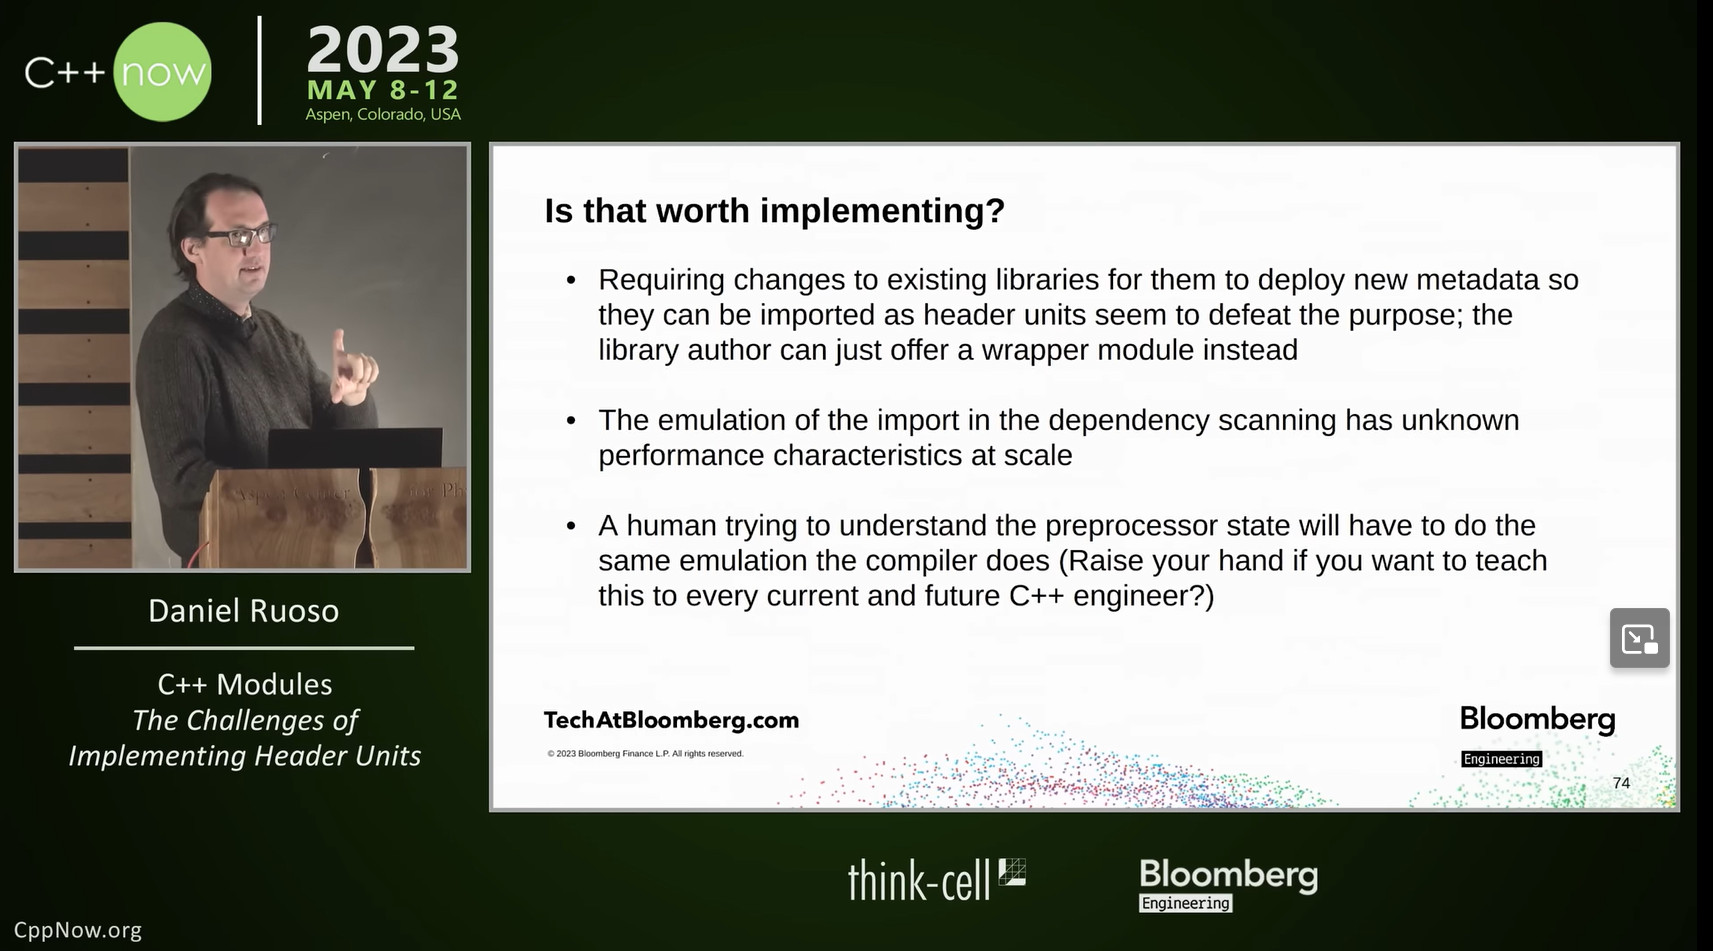
\includegraphics[height=.8\textheight]{modulesgfx/ruoso_header_units.jpg}}
  \end{center}
\end{frame}

\begin{frame}
  \frametitle{If you want to know more...}
  \small{Daniela Engert - So you want to use C++ Modules... cross-platform? (NDC TechTown 2023)}
  \begin{center}
    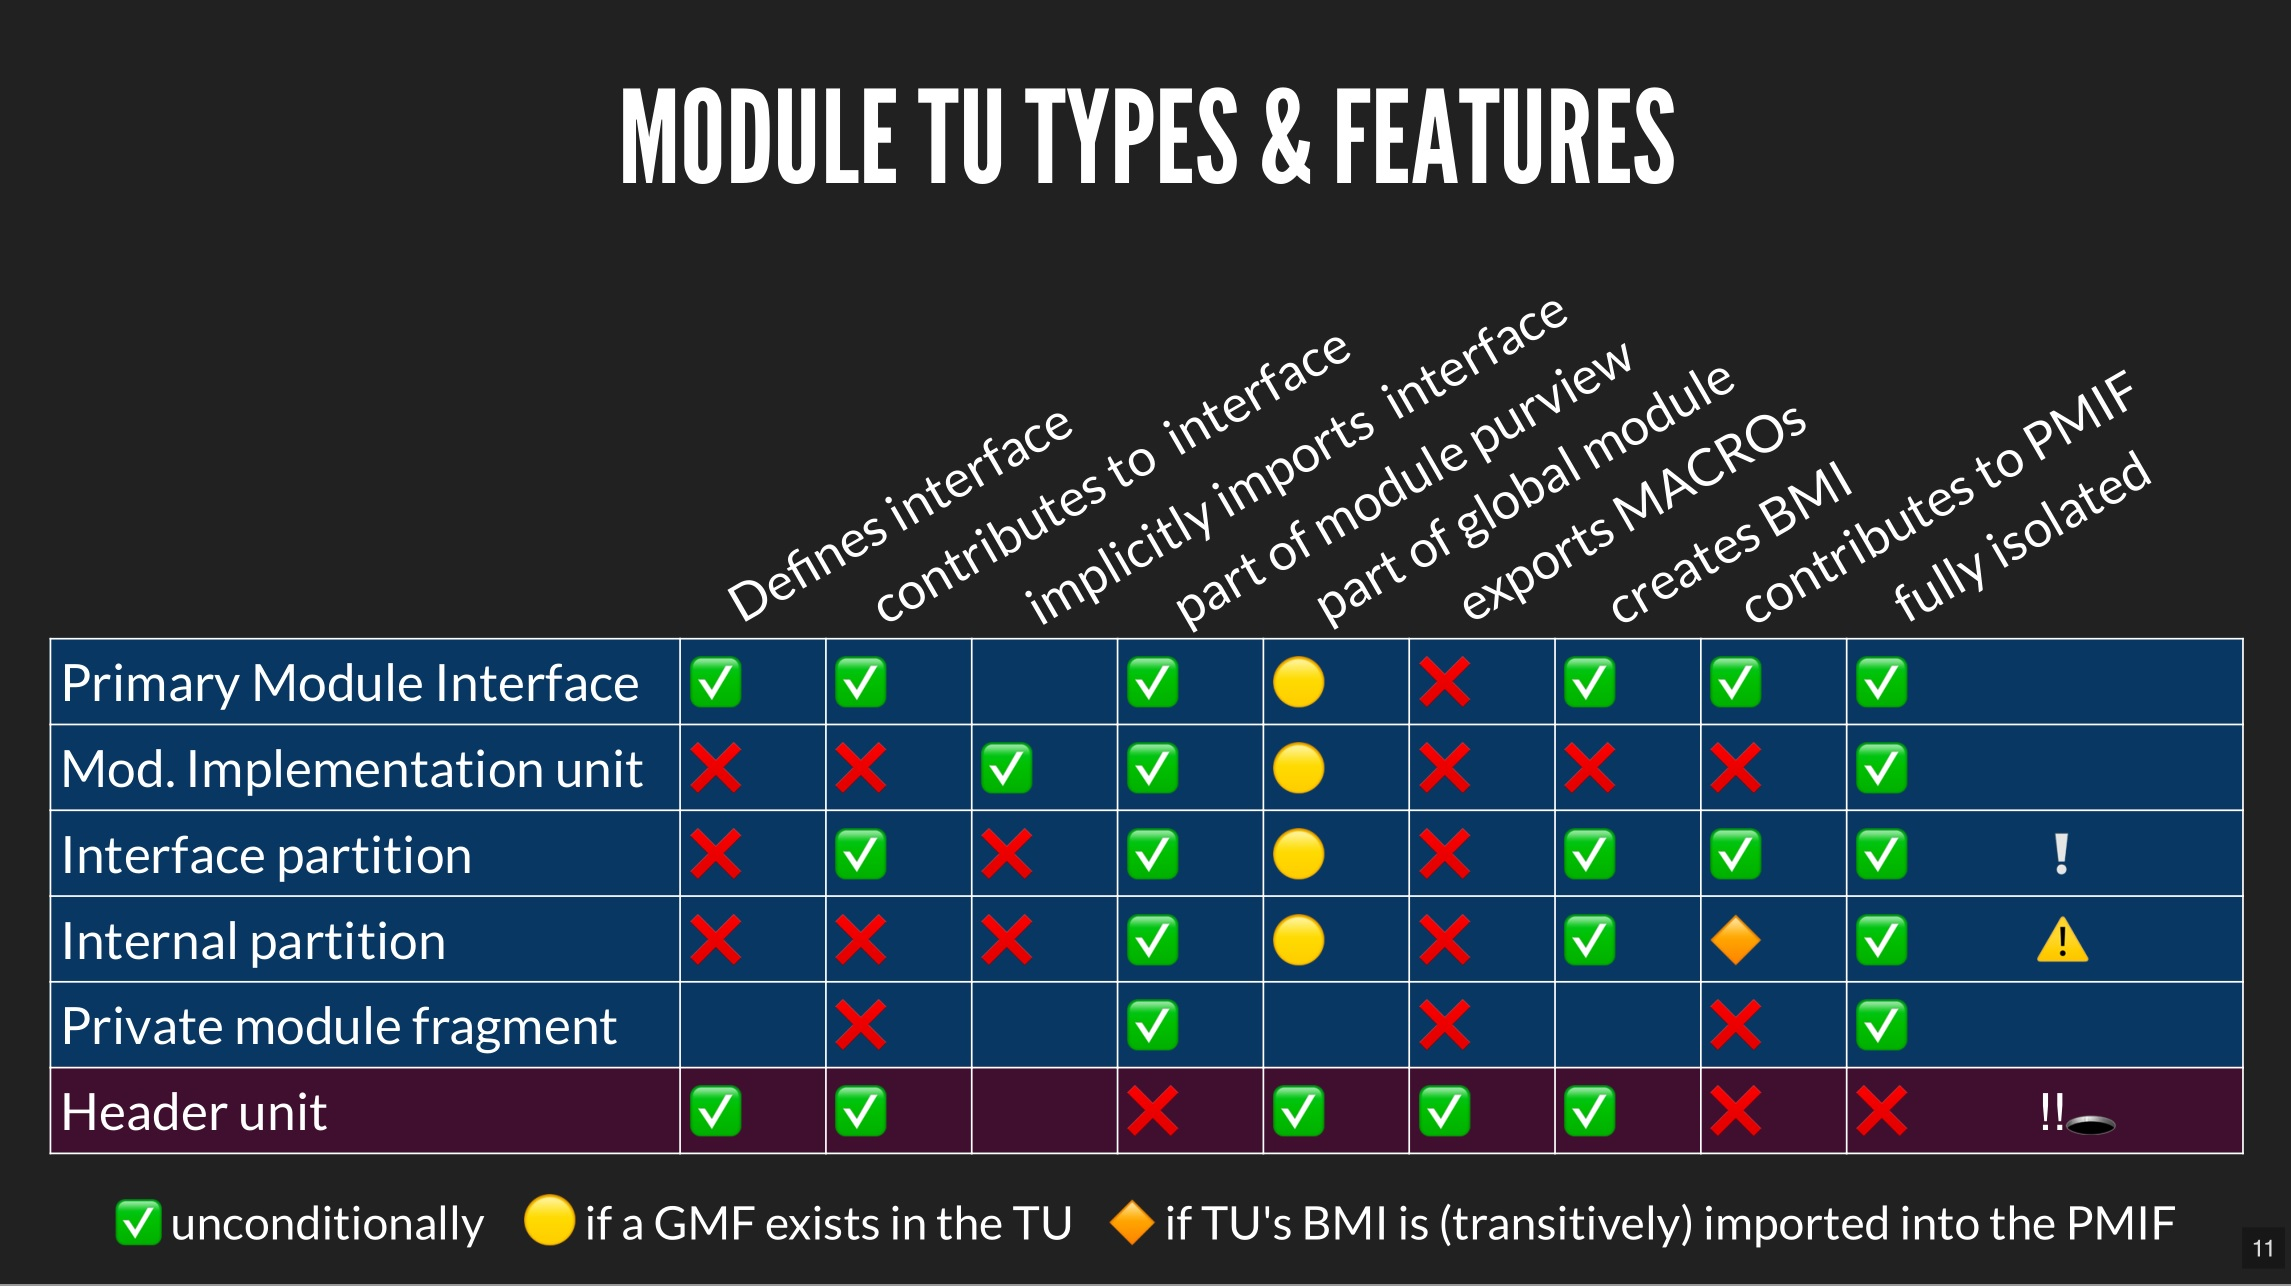
\includegraphics[height=.8\textheight]{modulesgfx/engert_table_new.jpg}
  \end{center}

  \note{
  \begin{itemize}
    \item I skipped some stuff; Watch one of Daniela's talks for more details
  \end{itemize}
  }
\end{frame}

\begin{frame}
  \frametitle{Building modules code with CMake}
  \note{
  \textbf{TIMECHECK}: 0:25
  }
\end{frame}

\begin{frame}[fragile]
  \frametitle{Building with CMake - Old School}

  \begin{lstlisting}[style=cmake]
cmake_minimum_required(VERSION 3.27)
project(my_project)

add_executable(my_executable)
target_sources(my_executable PUBLIC
  ${PROJECT_SOURCE_DIR}/my_src.cpp
  (*@\tmrk{a001}{}@*)${PROJECT_SOURCE_DIR}/inc/my_header1.hpp(*@\tmrk{b001}{}@*)
  (*@\tmrk{a002}{}@*)${PROJECT_SOURCE_DIR}/inc/my_header2.hpp(*@\tmrk{b002}{}@*)
)
target_include_directories(my_executable PUBLIC
  (*@\tmrk{a003}{}@*)${PROJECT_SOURCE_DIR}/inc(*@\tmrk{b003}{}@*))
  \end{lstlisting}

  \cuncover{2}{\tikz[overlay]\filldraw[blue, opacity=0.3] ([shift={(0,-0.5ex)}]a001) rectangle ([shift={(0,2ex)}]b001);}
  \cuncover{2}{\tikz[overlay]\filldraw[blue, opacity=0.3] ([shift={(0,-0.5ex)}]a002) rectangle ([shift={(0,2ex)}]b002);}
  \cuncover{3-}{\tikz[overlay]\filldraw[blue, opacity=0.3] ([shift={(0,-0.5ex)}]a003) rectangle ([shift={(0,2ex)}]b003);}

  \note{
  \begin{itemize}
    \item Old school CMake with headers
    \item Listing header sources only required for IDE
    \item Everything in include dir can be included
  \end{itemize}
  }
\end{frame}


\begin{frame}[fragile]
  \frametitle{Building with CMake - File Sets (since v3.23)}

  \begin{lstlisting}[style=cmake]
cmake_minimum_required(VERSION 3.27)
project(my_project)

add_executable(my_executable)
target_sources(my_executable PUBLIC
    ${PROJECT_SOURCE_DIR}/my_src.cpp
  PUBLIC
  (*@\tmrk{a010}{}@*)FILE_SET HEADERS(*@\tmrk{b010}{}@*)
  (*@\tmrk{a011}{}@*)BASE_DIRS(*@\tmrk{b011}{}@*) ${PROJECT_SOURCE_DIR}/inc
  (*@\tmrk{a012}{}@*)FILES(*@\tmrk{b012}{}@*)
    ${PROJECT_SOURCE_DIR}/inc/my_header1.hpp
    ${PROJECT_SOURCE_DIR}/inc/my_header2.hpp
)
  \end{lstlisting}

  \tikz[overlay]\filldraw[blue, opacity=0.3] ([shift={(0,-0.5ex)}]a010) rectangle ([shift={(0,2ex)}]b010);
  \tikz[overlay]\filldraw[blue, opacity=0.3] ([shift={(0,-0.5ex)}]a011) rectangle ([shift={(0,2ex)}]b011);
  \tikz[overlay]\filldraw[blue, opacity=0.3] ([shift={(0,-0.5ex)}]a012) rectangle ([shift={(0,2ex)}]b012);

  \note{
  \begin{itemize}
    \item New style file set
  \end{itemize}
  }
\end{frame}

\begin{frame}[fragile]
  \frametitle{Building with CMake - Modules (experimental as of v3.37)}

  \begin{lstlisting}[style=cmake]
cmake_minimum_required(VERSION 3.27)
project(my_project)
set((*@\tmrk{a015}{}@*)CMAKE_CXX_STANDARD 20(*@\tmrk{b015}{}@*))

add_executable(my_executable)
target_sources(my_executable PUBLIC
    ${PROJECT_SOURCE_DIR}/my_src.cpp
  PUBLIC
  (*@\tmrk{a010}{}@*)FILE_SET MODULES(*@\tmrk{b010}{}@*)
  (*@\tmrk{a011}{}@*)BASE_DIRS(*@\tmrk{b011}{}@*) ${PROJECT_SOURCE_DIR}/mod
  (*@\tmrk{a012}{}@*)FILES(*@\tmrk{b012}{}@*)
    ${PROJECT_SOURCE_DIR}/mod/my_module.cpp
)
  \end{lstlisting}

  \tikz[overlay]\filldraw[blue, opacity=0.3] ([shift={(0,-0.5ex)}]a010) rectangle ([shift={(0,2ex)}]b010);
  %\tikz[overlay]\filldraw[blue, opacity=0.3] ([shift={(0,-0.5ex)}]a011) rectangle ([shift={(0,2ex)}]b011);
  %\tikz[overlay]\filldraw[blue, opacity=0.3] ([shift={(0,-0.5ex)}]a012) rectangle ([shift={(0,2ex)}]b012);
  \tikz[overlay]\filldraw[blue, opacity=0.3] ([shift={(0,-0.5ex)}]a015) rectangle ([shift={(0,2ex)}]b015);

  \note{
  \begin{itemize}
    \item File set modules
  \end{itemize}
  }
\end{frame}

\begin{frame}[fragile]
  \frametitle{Some boilerplate required...}

  CMake Modules support is currently experimental. The details are boring and bound to change quickly.

  Refer to \underline{\href{https://stackoverflow.com/questions/57300495/how-to-use-c20-modules-with-cmake/61244367\#61244367}{https://t.ly/Dl8yE}} for the current state.

  \cpause
  \vspace{3em}
  For CMake 3.27 add:

  \begin{lstlisting}[style=cmake]
set(CMAKE_EXPERIMENTAL_CXX_MODULE_CMAKE_API
  aa1f7df0-828a-4fcd-9afc-2dc80491aca7)
  \end{lstlisting}
  For Clang you may also need to add:
  \begin{lstlisting}[style=cmake]
  set(CMAKE_CXX_EXTENSIONS OFF)
  \end{lstlisting}

  \note{
  \begin{itemize}
    \item Check StackOverflow, in particular if watching on YouTube
    \item Here is 3.27 for reference
  \end{itemize}
  }
\end{frame}

\begin{frame}
  \frametitle{Use the latest tools!}

  \begin{itemize}
  \item Absolute latest CMake (3.27)
  \item Latest Visual Studio 2022 (at least 19.34)
  \item Ninja 1.11
  \item Clang at least 17, prefer trunk
  \item gcc trunk
  \end{itemize}

  Even with the latest tools there are still plenty of bugs and inconsistent behavior between compilers!
\end{frame}


\begin{frame}[fragile]

  \frametitle{A few things to keep in mind}

  Module source file or regular source file?
  \begin{itemize}
  \item If it has an \texttt{export module} somewhere $\rightarrow$ Module
  \item If it is a module partition $\rightarrow$ Module
  \item Otherwise $\rightarrow$ Regular.
  \end{itemize}

  \cpause
  Which file extension?
  \begin{itemize}
  \item Many different extensions started appearing in the compilers: \texttt{.ixx}, \texttt{.cppm}, \texttt{.cxxm}, \texttt{.c++m}, \texttt{.ccm}.
  \item With CMake you don't need to use any of them!
  \item If you decide to use them, be sure to \textit{only} use them for module source files (as defined above)
  \end{itemize}

  \note{
  \begin{itemize}
    \item Module source or regular source
    \item File extensions
  \end{itemize}
  }
\end{frame}

\iffalse %!!!!!!!!!!!!!!!!!
\fi %!!!!!!!!!!!!!!!!!

\begin{frame}[fragile]
  \frametitle{What is a build system anyway?}

  \cpause
  \begin{lstlisting}
$ g++ -o my_src.o -I . -c my_src.cpp

$ g++ my_executable.o -o my_executable
  \end{lstlisting}

  \note{
  \textbf{TIMECHECK}: 0:35
  \begin{itemize}
  \item What's all this talk about build systems?
  \item We can just build from the command line!
  \end{itemize}
  }
\end{frame}

\begin{frame}

  \frametitle{Tracking dependencies}

  \begin{center}
  \only<1>{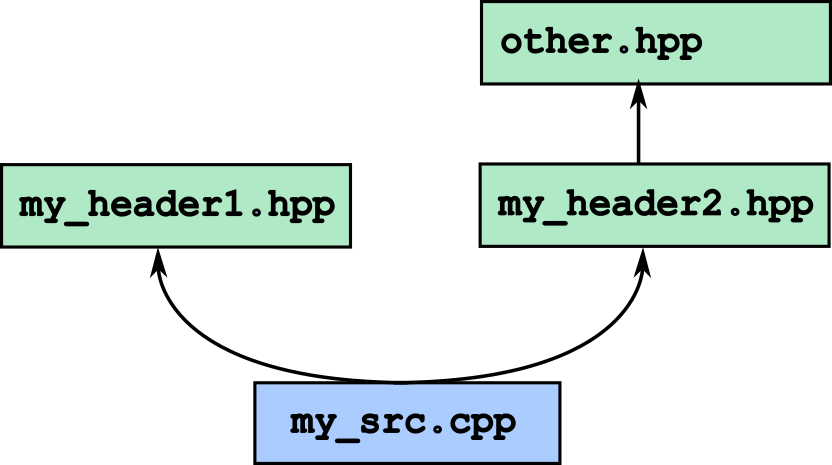
\includegraphics[height=.75\textheight]{modulesgfx/headers_dep_001.png}}
  \only<2>{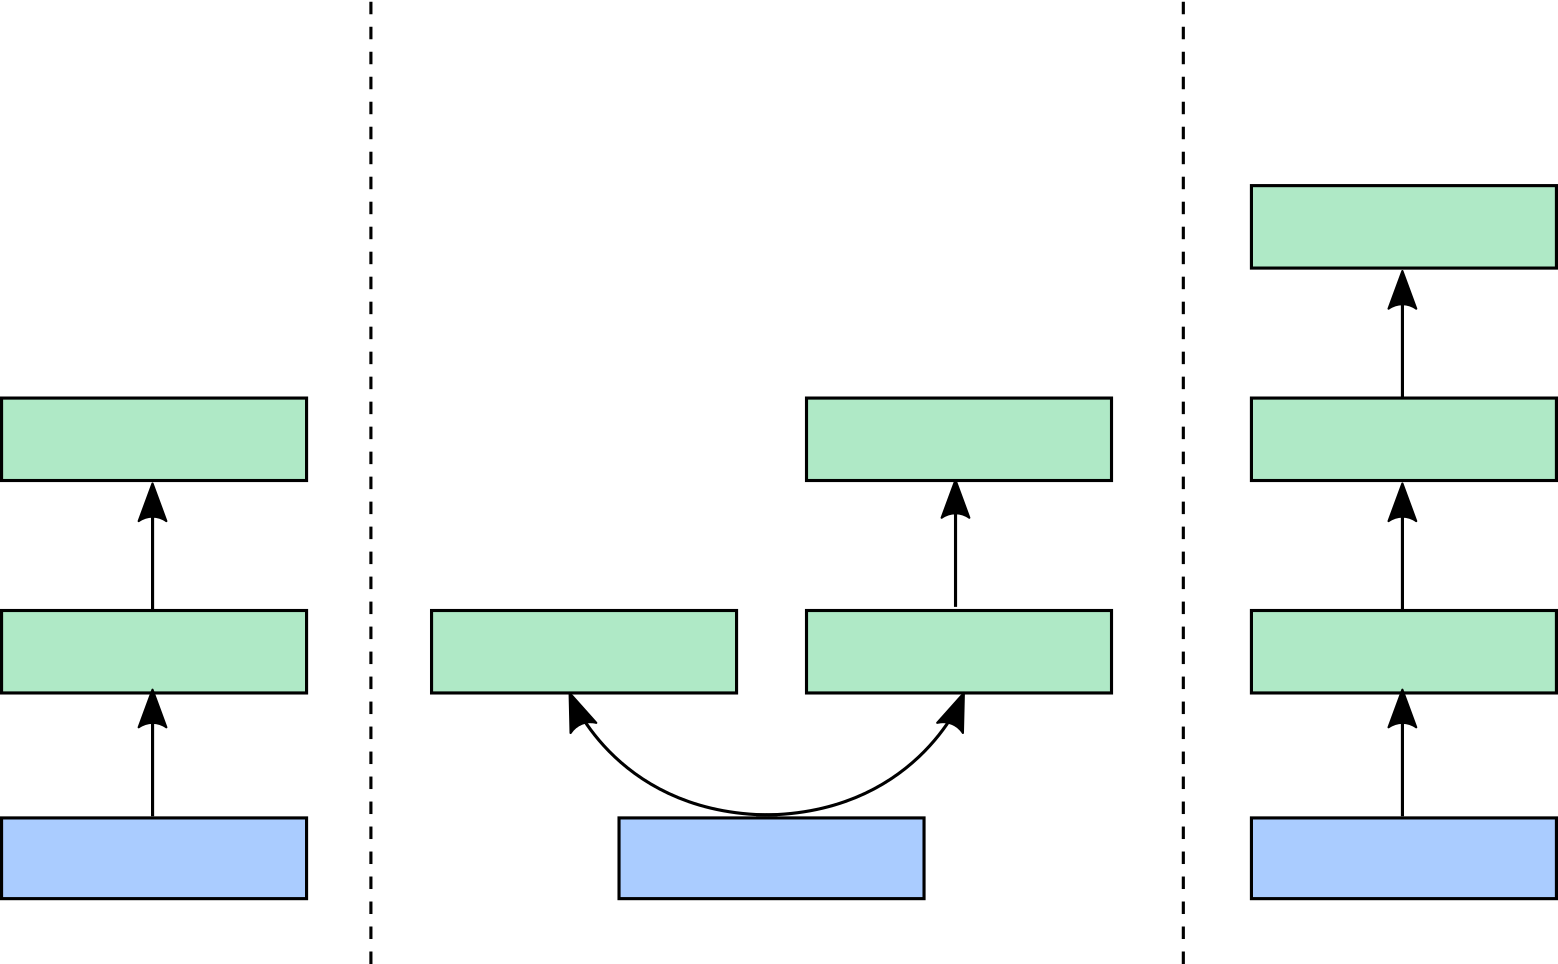
\includegraphics[height=.75\textheight]{modulesgfx/headers_dep_002.png}}
  \end{center}

  \note {
  \begin{itemize}
    \item Build system is a dependency tracker; if any header changes, I want affected sources to recompile
    \begin{itemize}
      \item Compiling too little means the program is incorrect
      \item Compiling too much is inefficient
    \end{itemize}
    \item This can be done independently for each source; Compiler can be invoked in parallel on all sources
  \end{itemize}
  How does the build system know which sources need rebuilding?
  }
\end{frame}

\begin{frame}[fragile]
  \frametitle{Tracking changes to header files}

  \begin{lstlisting}
$ g++ -o my_src.dep -I . -M -c my_src.cpp
  \end{lstlisting}

  \cpause

  --- \textit{File:} \texttt{my\_src.dep}
  \begin{lstlisting}
my_src.o: my_src.cpp \
  my_header1.hpp
  my_header2.hpp
  other.hpp
  \end{lstlisting}

  \note{
  How does the build system know which sources need rebuilding?
  \begin{itemize}
    \item Compiler writes out...
    \item Dependency file
  \end{itemize}
  }
\end{frame}

\begin{frame}[fragile]

  \frametitle{Tracking changes to header files}
  \only<1>{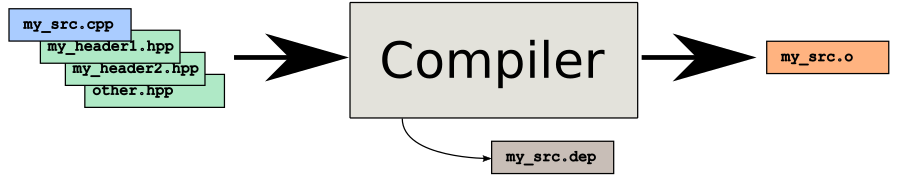
\includegraphics[width=.95\textwidth]{modulesgfx/compile_headers_001.png}}
  \iftransitions
  \only<2>{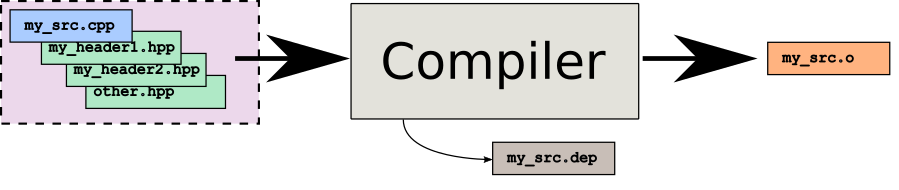
\includegraphics[width=.95\textwidth]{modulesgfx/compile_headers_002.png}}
  \only<3>{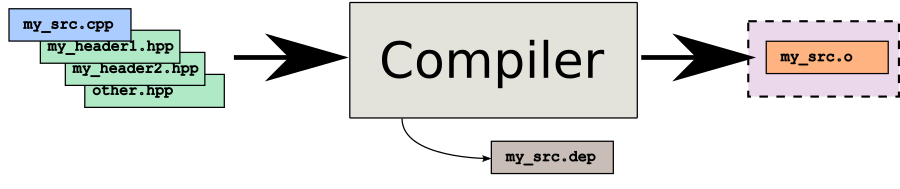
\includegraphics[width=.95\textwidth]{modulesgfx/compile_headers_003.png}}
  \only<4>{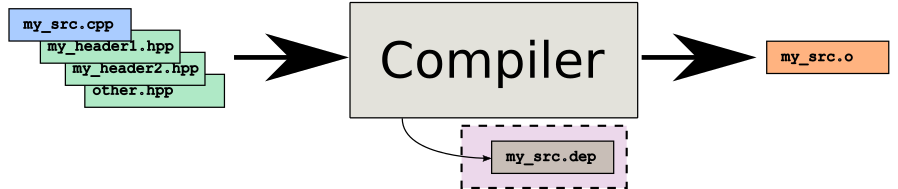
\includegraphics[width=.95\textwidth]{modulesgfx/compile_headers_004.png}}
  \fi

  \vspace{2em}
  \iftransitions
  \alert<4>{--- \textit{File:} \texttt{my\_src.dep}}
  \else
  --- \textit{File:} \texttt{my\_src.dep}
  \fi
  \begin{lstlisting}
my_src.o: my_src.cpp \
  my_header1.hpp
  my_header2.hpp
  other.hpp
  \end{lstlisting}

  \note{
  \begin{itemize}
    \item Compiler takes...
    \item As inputs sources and implicitly the included headers
    \item Produces as output the object file
    \item And the dependency file as byproduct; this is not used during subsequent build steps, just for the build system to track dependencies on incremental build
  \end{itemize}
  }
\end{frame}

\begin{frame}
  \begin{center}
  \frametitle{What changes for the build system?}
    \only<1>{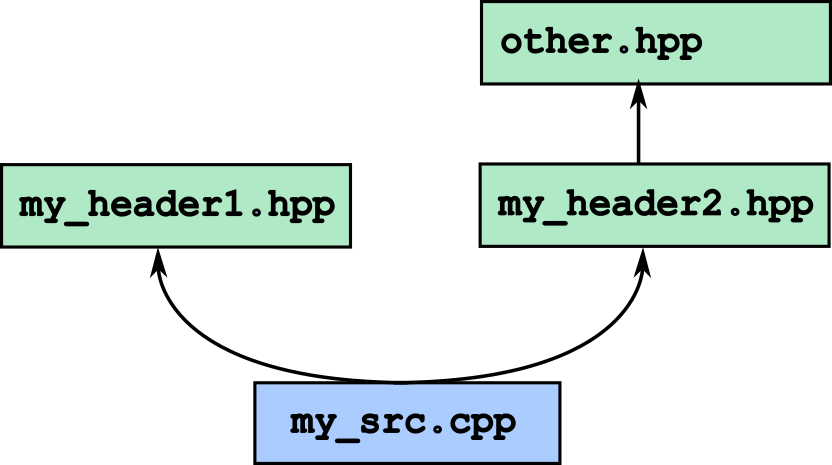
\includegraphics[height=.75\textheight]{modulesgfx/headers_dep_001.png}}
    \only<2>{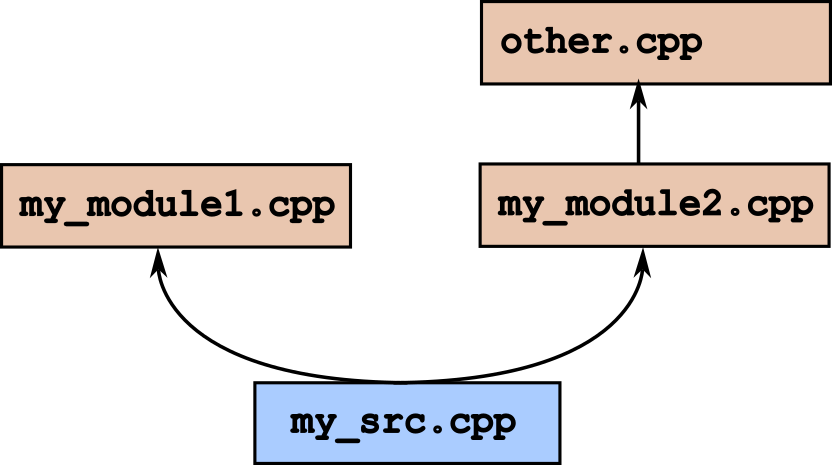
\includegraphics[height=.75\textheight]{modulesgfx/modules_dep_001.png}}
  \end{center}

  \note{
  \begin{itemize}
    \item What changes when switching from headers...
    \item to modules?
    \begin{itemize}
      \item We see right away sources now depend on sources.
    \end{itemize}
  \end{itemize}
  }
\end{frame}

\begin{frame}
  \frametitle{What changes for the build system?}

  \begin{center}
  \only<1>{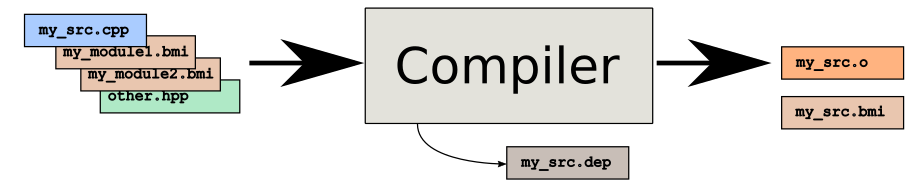
\includegraphics[width=.95\textwidth]{modulesgfx/modules_dep_010.png}}
  \iftransitions
  \only<2>{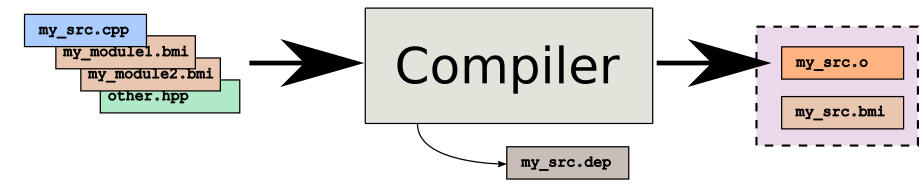
\includegraphics[width=.95\textwidth]{modulesgfx/modules_dep_012.png}}
  \only<3>{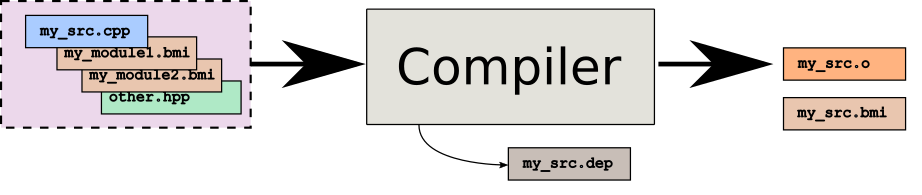
\includegraphics[width=.95\textwidth]{modulesgfx/modules_dep_011.png}}
  \fi
  \end{center}

  \note{
  \begin{itemize}
    \item Looking at the compiler...
    \item It now also produces a BMI output
    \item Compiler is still invoked per-source file but now takes bmis as implicit input as well
    \begin{itemize}
      \item BMI is not just a byproduct!
      \item Unlike dep file it is required for codegen of \texttt{my\_src.o}
    \end{itemize}
  \end{itemize}
  }
\end{frame}

\begin{frame}
  \begin{center}
  \frametitle{What changes for the build system?}
    \only<1>{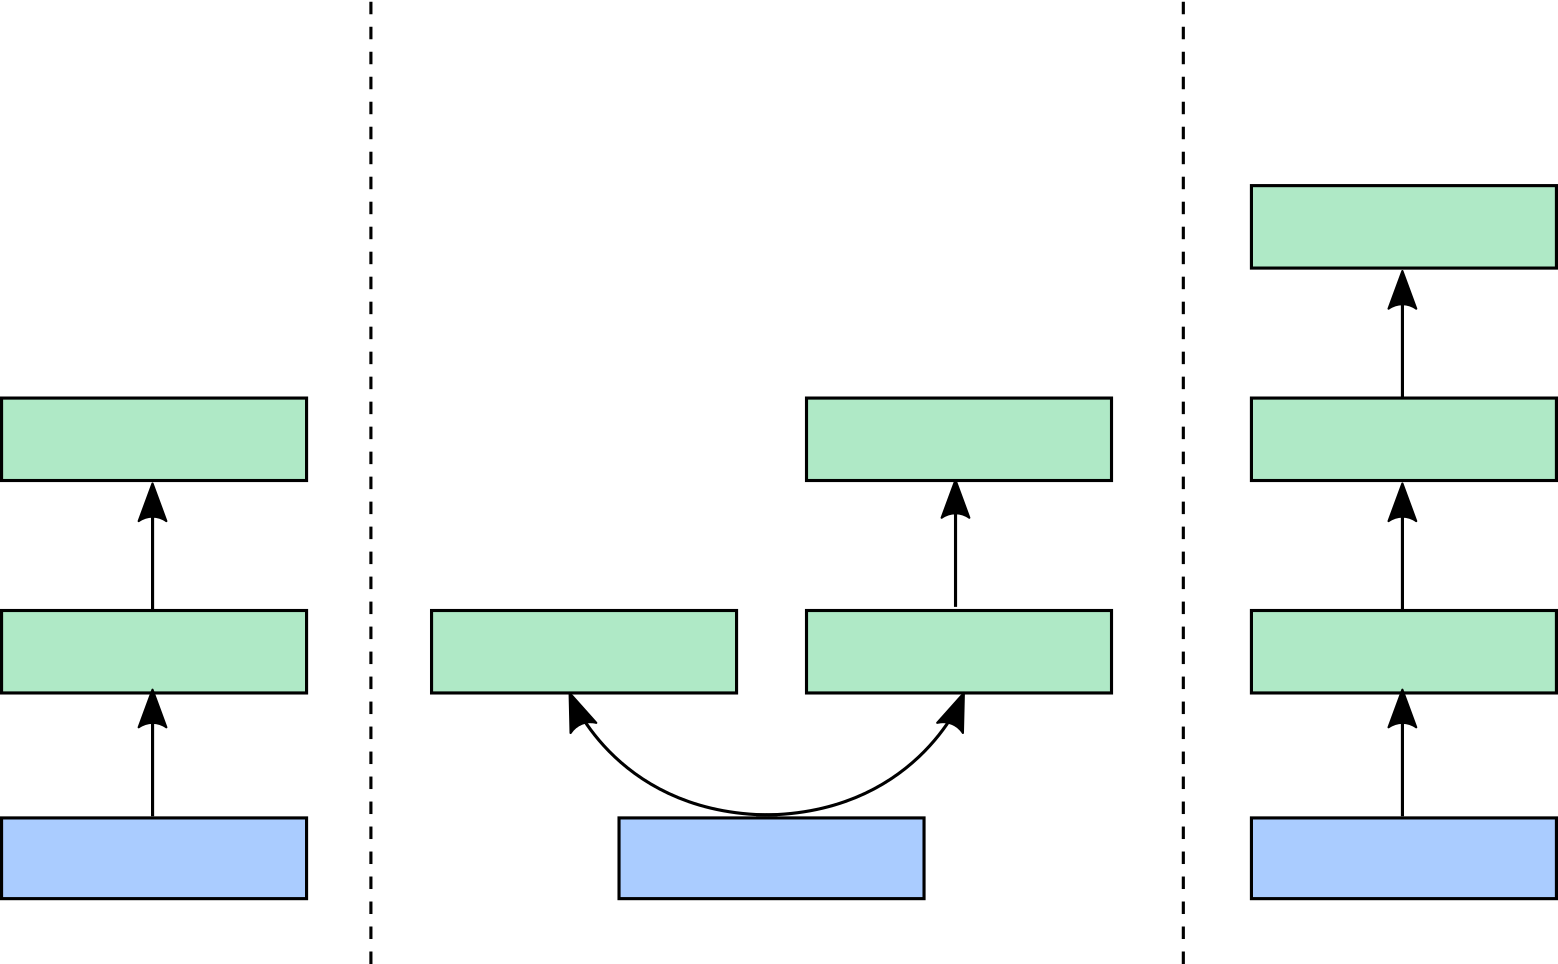
\includegraphics[height=.75\textheight]{modulesgfx/headers_dep_002.png}}
    \only<2>{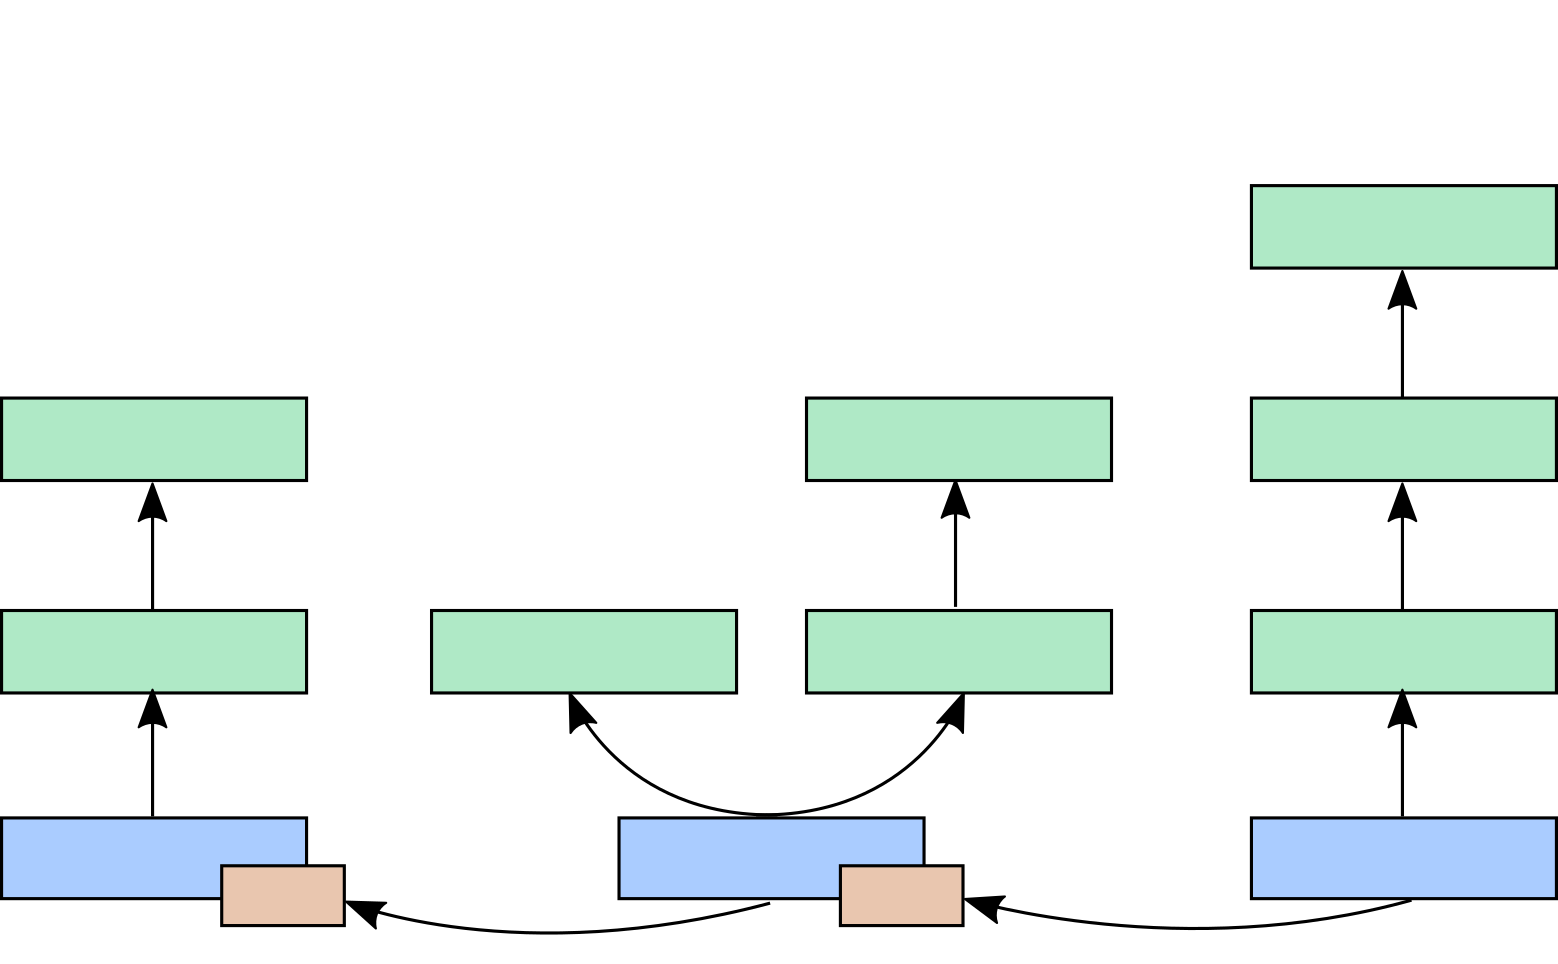
\includegraphics[height=.75\textheight]{modulesgfx/headers_dep_003.png}}
  \end{center}

  \note{
  \begin{itemize}
    \item Before each source file was compiled in isolation
    \item Now source file's depend on each other; to be exact, a source file depends on bmis of modules it imports
    \begin{itemize}
      \item Requires to build in order, according to dependencies
    \end{itemize}
  \end{itemize}
  }
\end{frame}

\begin{frame}[fragile]
  \frametitle{What changes for the build system?}

  \begin{onlyenv}<1>
    \begin{lstlisting}[style=cmake]
add_executable(my_executable)
target_sources(my_executable PUBLIC
    ${PROJECT_SOURCE_DIR}/my_src.cpp
  PUBLIC
  FILE_SET MODULES
  BASE_DIRS ${PROJECT_SOURCE_DIR}
  FILES
    (*@\tmrk{a050}{}@*)${PROJECT_SOURCE_DIR}/my_module1.cpp (*@\tmrk{b050}{}@*)
    (*@\tmrk{a051}{}@*)${PROJECT_SOURCE_DIR}/my_module2.cpp (*@\tmrk{b051}{}@*)
    (*@\tmrk{a052}{}@*)${PROJECT_SOURCE_DIR}/other.cpp      (*@\tmrk{b052}{}@*)
)
  \end{lstlisting}

  \tikz[overlay]\filldraw[blue, opacity=0.3] ([shift={(0,-0.5ex)}]a050) rectangle ([shift={(0,2ex)}]b050);
  \tikz[overlay]\filldraw[blue, opacity=0.3] ([shift={(0,-0.5ex)}]a051) rectangle ([shift={(0,2ex)}]b051);
  \tikz[overlay]\filldraw[blue, opacity=0.3] ([shift={(0,-0.5ex)}]a052) rectangle ([shift={(0,2ex)}]b052);
  \end{onlyenv}

  \begin{center}
  \only<2>{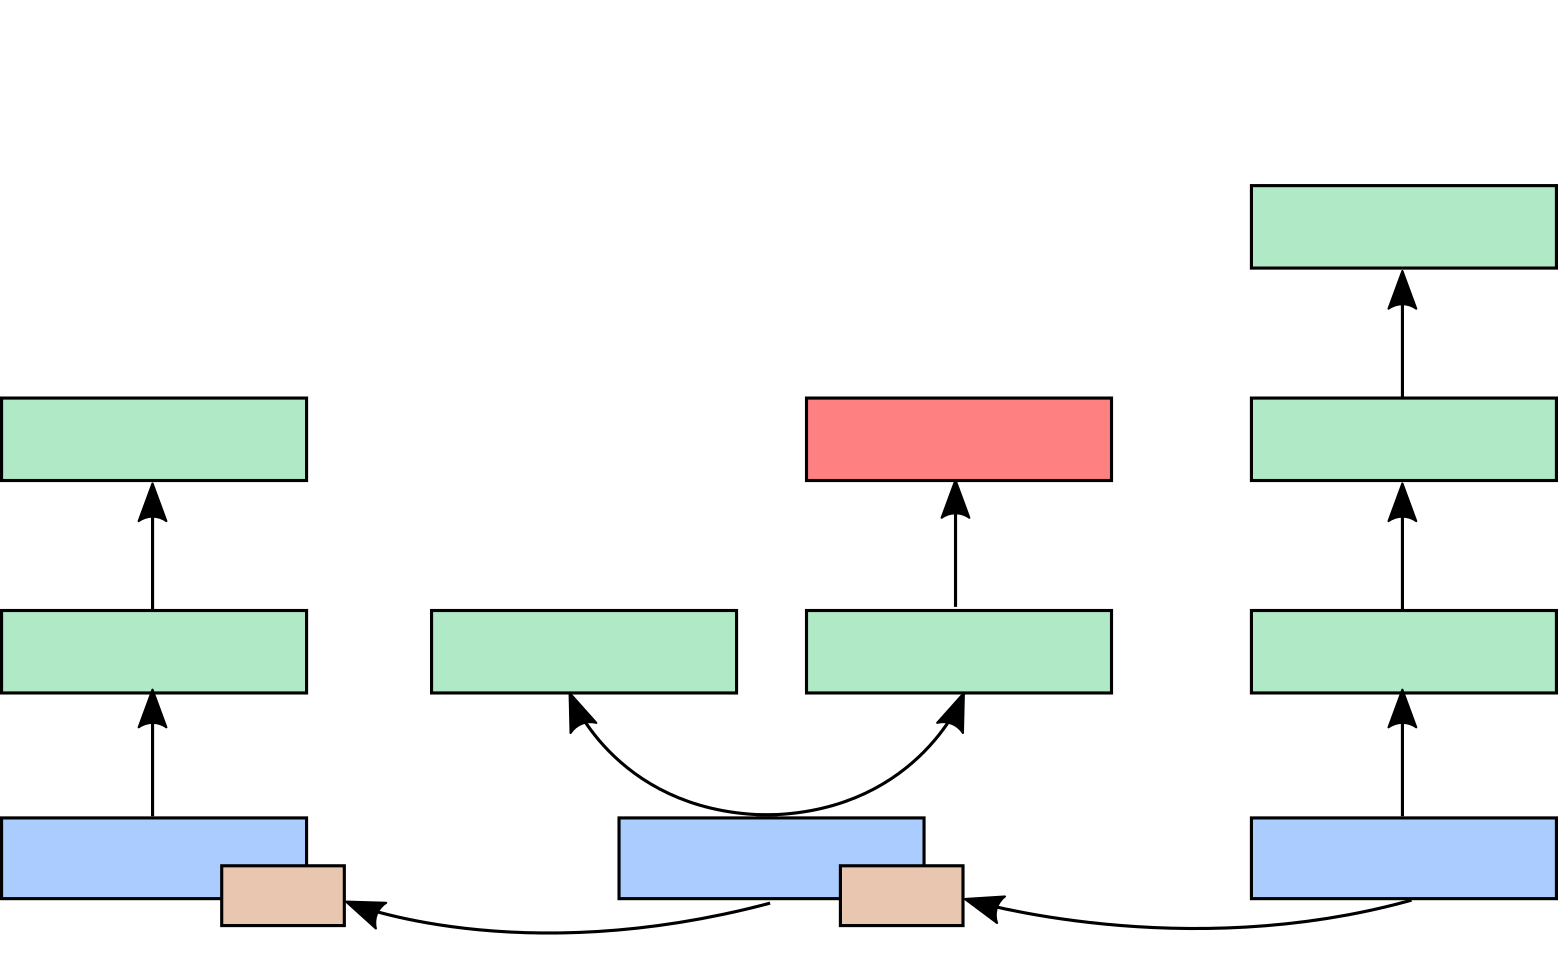
\includegraphics[height=.75\textheight]{modulesgfx/headers_dep_004.png}}
  \end{center}

  \note{
  \begin{itemize}
  \item In CMake: Source Files are listed individually, instead of directory
  \begin{itemize}
    \item But still just a flat list, no structure
    \item We don't want to model dependencies manually!
  \end{itemize}
  \item What do we need to rebuild if one file changes?
  \begin{itemize}
    \item Header dependencies apply as before
    \item Build system needs to run twice!
    \item First step just scans exports and imports
    \item Second step compiles in right order creating object and bmi files
    \item Touching header causes middle and right branch to recompile; but middle has to compile first
  \end{itemize}
  \end{itemize}
  }
\end{frame}

\begin{frame}
  \frametitle{Some useful advice for starting out...}

  \begin{center}
  \includegraphics[height=.90\textheight]{modulesgfx/its_dangerous_to_go_alone.png}
  \end{center}
  \note{
  \textbf{TIMECHECK}: 0:45
  }
\end{frame}


\begin{frame}[fragile]
  \frametitle{Interacting with headers - the global module fragment}

  \begin{onlyenv}<1-2>
  \begin{lstlisting}[style=cpp20]
export module A;

(*@\tmrk{a060}{}@*)import std;(*@\tmrk{b060}{}@*)

export std::vector<int> getVector() {
  return std::vector<int>{ 1, 2, 3, 4 };
}
  \end{lstlisting}
  \end{onlyenv}

  \only<1>{
  \tikz[overlay]\filldraw[blue, opacity=0] ([shift={(0,-0.5ex)}]a060) rectangle ([shift={(0,2ex)}]b060);
  }
  \only<2>{
  \tikz[overlay]\filldraw[blue, opacity=0.3] ([shift={(0,-0.5ex)}]a060) rectangle ([shift={(0,2ex)}]b060);
  }

  \begin{onlyenv}<3-6>
  \begin{lstlisting}[style=cpp20]
(*@\tmrk{a061}{}@*)module;(*@\tmrk{b061}{}@*)

(*@\tmrk{a065}{}@*)#include <vector>(*@\tmrk{b065}{}@*)

(*@\tmrk{a062}{}@*)export module A;(*@\tmrk{b062}{}@*)

(*@\tmrk{a066}{}@*)export std::vector<int> getVector() {(*@\tmrk{b066}{}@*)
(*@\tmrk{a067}{}@*)  return std::vector<int>{ 1, 2, 3, 4 };(*@\tmrk{b067}{}@*)
(*@\tmrk{a068}{}@*)}(*@\tmrk{b068}{}@*)
  \end{lstlisting}
  \end{onlyenv}
  \only<3>{
  \tikz[overlay]\filldraw[blue, opacity=0] ([shift={(0,-0.5ex)}]a061) rectangle ([shift={(0,2ex)}]b061);
  }
  \only<4-6>{
  \tikz[overlay]\filldraw[blue, opacity=0.3] ([shift={(0,-0.5ex)}]a061) rectangle ([shift={(0,2ex)}]b061);
  \tikz[overlay]\filldraw[blue, opacity=0.3] ([shift={(0,-0.5ex)}]a062) rectangle ([shift={(0,2ex)}]b062);
  }
  \only<5>{
  \tikz[overlay]\filldraw[red, opacity=0.3] ([shift={(0,-0.5ex)}]a065) rectangle ([shift={(0,2ex)}]b065);
  }
  \only<6>{
  \tikz[overlay]\filldraw[green, opacity=0.3] ([shift={(0,-0.5ex)}]a066) rectangle ([shift={(0,2ex)}]b066);
  \tikz[overlay]\filldraw[green, opacity=0.3] ([shift={(0,-0.5ex)}]a067) rectangle ([shift={(0,2ex)}]b067);
  \tikz[overlay]\filldraw[green, opacity=0.3] ([shift={(0,-0.5ex)}]a068) rectangle ([shift={(0,2ex)}]b068);
  }

  \note {
  \begin{itemize}
  \item Simple, ideal world...
  \item Everything is modules.
  \item If we need headers things change...
  \item We put \texttt{module;} at the top...
  \item Everything between is GMF; put all \texttt{\#include}s here, but no import!
  \item Everything after export is \textit{model purview}
  \end{itemize}
  }
\end{frame}

\begin{frame}[fragile]
  \frametitle{Beware of mixing headers and modules}
  --- \textit{File:} \texttt{my\_module.cpp}
  \begin{lstlisting}[style=cpp20]
export module m;

import std;

export std::string f() { return "!"; }
  \end{lstlisting}
  \cpause
  --- \textit{File:} \texttt{main.cpp}
  \begin{onlyenv}<1-2>
  \begin{lstlisting}[style=cpp20]
import m;


int main() {
  auto const s = f();
}
  \end{lstlisting}
  \end{onlyenv}
  \begin{onlyenv}<3>
  \begin{lstlisting}[style=cpp20]
import m;


int main() {
  std::string const s = f();
}
  \end{lstlisting}
  \end{onlyenv}
  \begin{onlyenv}<4>
  \begin{lstlisting}[style=cpp20]
import m;
#include <string>

int main() {
  std::string const s = f();
}
  \end{lstlisting}
  \end{onlyenv}

  \note{
  \begin{itemize}
    \item I import std but don't export...
    \item Client does not know name of \texttt{std::string}; \texttt{auto} works...
    \item But this does not. So let's include to get the name?
    \item No, this also does not work. Header string is a different name than module string!
  \end{itemize}
  Avoid mixing headers and modules!
  }
\end{frame}

\begin{frame}[fragile]
  \frametitle{When mixing, always put \texttt{\#includes} first!}

  \begin{lstlisting}[style=cpp20]
#include <string>

// Guideline: All #includes should
//  come before the first import!
import std;
  \end{lstlisting}

  \begin{lstlisting}[style=cpp20]

int main() {
  std::string const s = f();
}
  \end{lstlisting}
  \note{
  If you must, follow this guideline. Should work for std.

  Prefer not mixing.
  }
\end{frame}

\begin{frame}[fragile]
  \frametitle{Modularizing legacy libraries - Include standard library early}
  --- \textit{File:} \texttt{lib.hpp}
  \begin{lstlisting}[style=cpp20]
#include <string>
std::string f();
  \end{lstlisting}

  \begin{onlyenv}<1>
  --- \textit{File:} \texttt{libm.cpp}
  \begin{lstlisting}[style=cpp20]



export module lib;
export {
#include <lib.hpp>
}
  \end{lstlisting}
  \end{onlyenv}

  \begin{onlyenv}<2>
  --- \textit{File:} \texttt{libm.cpp}
  \begin{lstlisting}[style=cpp20]
module;
#include <string>

export module lib;
export {
#include <lib.hpp>
}
  \end{lstlisting}
  \end{onlyenv}

  \note{
  \begin{itemize}
    \item Let's say we export something that uses std
    \item Include std in GMF will prevent include happening in export
  \end{itemize}
  }
\end{frame}

\begin{frame}[fragile]
  \frametitle{Modularizing legacy libraries - Export names with \texttt{using}}

  --- \textit{File:} \texttt{lib.hpp}
  \begin{lstlisting}[style=cpp20]
class AwesomeType;
  \end{lstlisting}
  --- \textit{File:} \texttt{libm.cpp}
  \begin{lstlisting}[style=cpp20]
module;
#include <lib.hpp>
export module lib;
export using ::AwesomeType;
  \end{lstlisting}

  \note {
  Include in GMF, export what is needed with using.
  }
\end{frame}

\begin{frame}[fragile]
  \frametitle{Modularizing legacy libraries - Preprocessor macros}

  --- \textit{File:} \texttt{libm.cpp}
  \begin{lstlisting}[style=cpp20]
export module lib;
#define AWESOME_MACRO 42
  \end{lstlisting}

  --- \textit{File:} \texttt{main.cpp}
  \begin{lstlisting}[style=cpp20]
import lib;

int main() {
  return AWESOME_MACRO;  // error! macros
                         // cannot be exported
}
  \end{lstlisting}

  \note{
  For macros...
  }
\end{frame}

\begin{frame}[fragile]
  \frametitle{Modularizing legacy libraries - Preprocessor macros}

  --- \textit{File:} \texttt{libm.cpp}
  \begin{lstlisting}[style=cpp20]
export module lib;
// ...
  \end{lstlisting}

  --- \textit{File:} \texttt{libm.hpp}
    \begin{lstlisting}[style=cpp20]
#define AWESOME_MACRO 42
  \end{lstlisting}

  --- \textit{File:} \texttt{main.cpp}
  \begin{lstlisting}[style=cpp20]
#include <libm.hpp>
import lib;

int main() {
  return AWESOME_MACRO;
}
  \end{lstlisting}

  \note{
  Have separate header
  }
\end{frame}


\begin{frame}[fragile]
  \frametitle{Modularizing legacy libraries - Preprocessor macros}

  --- \textit{File:} \texttt{libm.cpp}
  \begin{lstlisting}[style=cpp20]
export module lib;
#define AWESOME_MACRO 42
export constexpr int AwesomeConstant =
    AWESOME_MACRO;
  \end{lstlisting}

  --- \textit{File:} \texttt{main.cpp}
  \begin{lstlisting}[style=cpp20]
import lib;

int main() {
  return AwesomeConstant;
}
  \end{lstlisting}

  \note{
  Or provide non-preprocessor alternative in module
  }
\end{frame}

\begin{frame}
  \frametitle{Daniela Engert - Contemporary C++ in Action}
  \begin{center}
    \href{https://www.youtube.com/watch?v=yUIFdL3D0Vk}
    {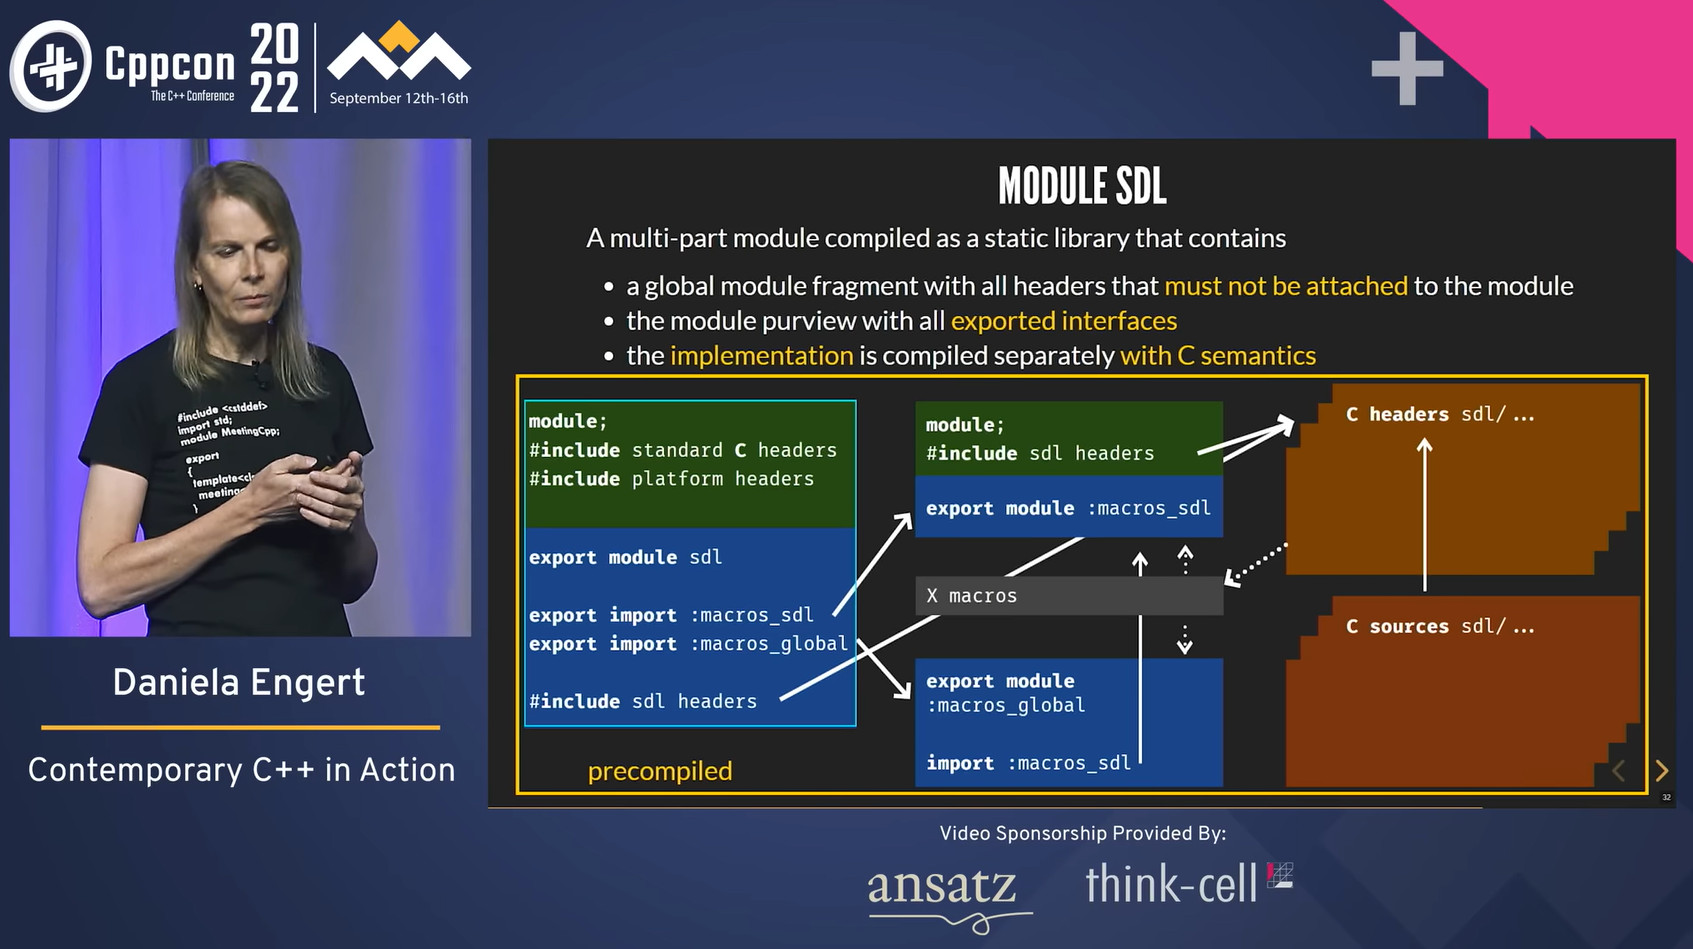
\includegraphics[height=.8\textheight]{modulesgfx/engert_contemporary.jpg}}
  \end{center}
\end{frame}


\begin{frame}
  \frametitle{Conclusion}

  \begin{itemize}
  \item Modules are slowly maturing. Try them out today!
  \item There is still a lot of dark corners in the implementations, but the more people use them, the quicker those get fixed.
  \item Integrating header-based legacy code is challenging and requires some
  practice.
  \item \alert<2>{There is a lot of low-hanging fruit there for people interested in contributing to compilers and tooling}
  \end{itemize}

  \note{
  \begin{itemize}
    \item Try it; Still bugs; Beware legacy
    \item Implementation opportunities!
  \end{itemize}
  \textbf{TIMECHECK}: 0:55
  }
\end{frame}

\begin{frame}
  \frametitle{Where to go from here...}

  \begin{itemize}
    \item Luis Caro Campos - C++20 Modules: The Packaging and Binary Redistribution Story (CppCon 2023, right afterwards in Cottonwood)
    \vspace{1em}
    \item \href{https://www.youtube.com/watch?v=Kqo-jIq4V3I}{Daniela Engert - Modules: The Beginner's Guide (Meeting C++ 2019)}
    \item \href{https://www.youtube.com/watch?v=nP8QcvPpGeM}{Daniela Engert - A Short Tour of C++ Modules (CppCon 2021)}
    \item \href{https://www.youtube.com/watch?v=c563KgO-uf4}{Bill Hoffman - import CMake: 2023 State of C++20 modules in CMake (CppNow 2023)}
    \item \href{https://www.youtube.com/watch?v=IZXNsim9TWI}{Bret Brown - Modern CMake Modules (CppCon 2021)}
    \item \href{https://vector-of-bool.github.io/2019/03/10/modules-1.html}{vector-of-bool - Understanding C++ Modules (Blog post series)}
    \item \href{https://mathstuf.fedorapeople.org/fortran-modules/fortran-modules.html}{Boeckel, King, Maynard, Hoffman - How CMake supports Fortran modules and its applicability to C++ (WG21 D1483)}
  \end{itemize}
\end{frame}

% @todo: Other modules talks

\begin{frame}
  \frametitle{Thanks for your attention.}

  \href{https://stackoverflow.com/users/577603/comicsansms}{
\includegraphics[height=.05\textheight]{resources/so-icon.png}}
  \href{https://github.com/ComicSansMS}{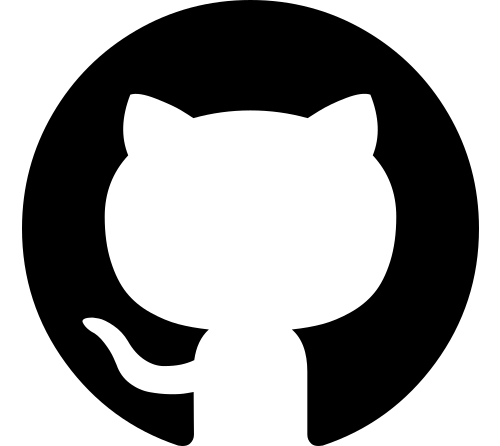
\includegraphics[height=.05\textheight]{resources/github-icon.png}}
  \includegraphics[height=.05\textheight]{resources/discord-icon.png} Andreas Weis
\end{frame}


\end{document}
